\chapter{Result}  \label{sec::Result}
After fixing the background estimation algorithm, the data in the signal regions are unblinded.
The yields are compared with either the background-only hypothesis or various signal hypothesis,
testing the compatibility.
The statistical result is finally interpretated into physics results, in a form of exclusion limit in terms of the SUSY masses either the cross-section upper limits. \\

This chapter begins with describing the statistical procedure employed in deriving the background expectation (i.e. deciding the normalization factors in the kinematical extrapolation) and the hypothesis tests. Unblinded data in the signal regions are then shown, and the statistical result and the interpretation are discussed in the end of this chapter.


\section{Statistical Analysis and Hypothetical Test} \label{sec::Result::statistics}
\paragraph{Profile likelihood and treatment of systematics} 
Statistical tests are performed to examine the consistency of observed data with respect to the SM background expectation or that with specific signal being overlaid. 
This is implemented via a likelihood function based on the probability density distribution (PDF) in terms of number of observed events in each signal region bin. 
The full representation of the likelihood is given by Eq. (\ref{eq::Result::LH}):
\begin{align}
 \mathcal{L} (\mu; \muw, \mutop, \bmtheta)  
 & =  \mathcal{L} ( \bm{n}^{\SR}, \bm{n}^{\WR}, \bm{n}^{\TR} | \mu, \muw, \mutop, \bmtheta) \nn \\
  & = \mathcal{P}_{\SR} \times \mathcal{P}_{\CR}  \times \prod_{k\in \mathrm{syst.}} \rho(\theta_k), \nn \\
& \nn \\
% 
  \mathcal{P}_{\SR} & = \prod_{i\notin \textbf{3B}} \,\, \left[ \prod_{b \in \mathrm{BT}, \mathrm{BV}} \,\, \mathrm{Pois}\, (n^{\SR}_{i,b} | \mu s^{\SR}_{i,b}(\bmtheta) + \muw \,  w^{\SR}_{i,b}(\bmtheta) + \mutop \,  t^{\SR}_{i,b}(\bmtheta) + b^{\SR}_{i,b}(\bmtheta)) \right] \nn \\
& \times \prod_{i\in \textbf{3B}} \,\, \mathrm{Pois}\, (n^{\SR}_i | \mu s^{\SR}_i(\bmtheta) + \muw \,  w^{\SR}_i(\bmtheta) + \mutop \,  t^{\SR}_i(\bmtheta) + b^{\SR}_i(\bmtheta))  \nn \\
& \nn\\
%
  \mathcal{P}_{\CR} =  \prod_i \,\,
  &        \mathrm{Pois}\, (n^{\TR}_i | \mu s^{\WR}_i(\bmtheta) + \muw \,  w^{\WR}_i(\bmtheta) + \mutop \,  t^{\WR}_i(\bmtheta) + b^{\WR}_i(\bmtheta))  \nn \\
  & \times \mathrm{Pois}\, (n^{\WR}_i | \mu s^{\TR}_i(\bmtheta) + \muw \,  w^{\TR}_i(\bmtheta) + \mutop \,  t^{\TR}_i(\bmtheta) + b^{\TR}_i(\bmtheta))   
\label{eq::Result::LH}
\end{align}
where $\bm{n}^{\SR}$, $\bm{n}^{\WR}$ and $\bm{n}^{\TR}$ are respectively the numbers of observed events in SRs, corresponding CRs such as WRs and TRs, with the vector indices running over regions ;
$s_{r}$ is the expected signal yield in region $r$ in the signal model to be tested;
$w_{r}$ and $t_{r}$ are respectively the expectedyields of $\wjets$ and the top backgroud in region $r$ before the normalization, with the components derived by the object replacement method being excluded;
$b_{r}$ are the expectedyields of the other backgrounds in region $r$;
$\bmtheta$ is the vector of nuisance parameters for each systematic uncertainty; 
$\muw$ and $\mutop$ are the normalization factors for $\wjets$ and the top backgroud which are allowed to vary between $i$; 
and $\mu$ is the signal strength, a parameter describing the relative normalization with respect to the signal model to be tested i.e. $\mu=0$ corresponds to a background-only hypothesis and $\mu=1$ to a hypothesis with the nominal signal level expected by the signal model. Index $i$ runs along signal region bins joining the combination that are orthogonal to each other s.t. :
%
\begin{align}
i \in \,\, \{ \,\,\, & \textbf{2J},\textbf{6J},\textbf{3B}  \,\,\, \}  \nn \\
\mbox{ or } & \{ \,\, \textbf{2J},\textbf{High-x},\textbf{3B} \,\,\}  \nn \\
\mbox{ or } & \{ \,\, \textbf{Low-x},\textbf{6J},\textbf{3B} \,\,\}  \nn \\
\mbox{ or } & \{ \,\, \textbf{Low-x},\textbf{High-x},\textbf{3B} \,\,\}
\end{align}
where
\begin{align}
\textbf{2J} & = \,\, \{ \,\,\, \mbox{2J-$\meffIncFirst$, 2J-$\meffIncSecond$, 2J-$\meffIncThird$}  \,\,\, \}  \nn \\
\textbf{6J} & = \,\, \{ \,\,\, \mbox{6J-$\meffIncFirst$, 6J-$\meffIncSecond$, 6J-$\meffIncThird$}  \,\,\, \}  \nn \\
\textbf{Low-x} & = \,\, \{ \,\,\, \mbox{Low-x}  \,\,\, \}  \nn \\
\textbf{High-x} & = \,\, \{ \,\,\,\mbox{High-x}   \,\,\, \}  \nn \\
\textbf{3B} & = \,\, \{ \,\,\, \mbox{3B-$\meffIncFirst$, 3B-$\meffIncSecond$}  \,\,\, \}  \nn \\
\end{align}

The normalization factors for $\wjets$ and the top background backgrounds are simultaneously determined,
in order to correlate the behavior of systematics.
Therefore the CRs terms are also placed in the common likelihood with an identical representation as SRs. \\

The statistical behavior of the PDFs is fully characterized by a product of Poisson distributions for each SR or CR:
\begin{align}
\mathrm{Pois}\,(n|\nu) & := \frac{\nu^n}{n!} e^{-\nu} \nn
\end{align}
where $\nu$ and $n$ are the expected yield and observed number respectively. \\

The effect of a systematics (indexed by $k$) are then incorporated by shifting the Poisson mean $\nu$, via a corresponding nuisance parameter $\theta_k$ so as:
$\nu(0)$ corresponds to the nominal expectation and $\nu(\pm1)$ to that with $\pm 1\sigma$ variation due to the systematics. 
While $\nu(0)$ and $\nu(\pm1)$ are calculated explicitly, the whole function $\nu(\theta_k)$ is obtained by interpolating or extrapolating the three points using a polynomial or an exponential function, providing a continuous functional form of $\mathcal{L}$ in terms of $\bmtheta$. \\

What is here intend to do is to perform a global fit on data, simultaneously determining $\mu, \muw, \mutop$ and $\bmtheta$ by minimizing the likelihood $\mathcal{L}$ (Eq. \ref{eq::Result::LH}). While $\mu, \muw$ and $\mutop$ are allowed to flow based on our total ignorance, the shifts of the nuisance parameters $\bmtheta$ need to be restricted reflecting the level of our confidence. This is implemented by the last terms in the likelihood $\prod_{k \in \mathrm{syst.}} \rho(\theta_k)$ known as the ``penalty terms'' serving as the prior constraints for the likelihood. 
The form of the penalty terms depends on the statistical nature of each systematics:
\begin{itemize}
%jav. need to change
\item A Gaussian PDF is commonly assumed for most systematic uncertainties:
\begin{align}
%\rho (\theta) = \frac{1}{\sqrt{2\pi}\sigma} \mathrm{exp} \left( - \frac{(\theta-\hat{\theta})^2}{2\sigma^2} \right)
\rho (\theta) = \frac{1}{\sqrt{2\pi}\sigma} \mathrm{exp} \left( - \frac{\theta^2}{2} \right)
\end{align}

%\begin{align}
%\rho (\theta) = \frac{1}{\sqrt{2\pi}\log{\sigma}} \mathrm{exp} \left( - \frac{(\log{(\theta/\hat{\theta})})^2}{2(\log{\sigma})^2} \right) \frac{1}{\theta}
%\end{align}

\item The Gamma PDF is used to describe uncertainties following according to Poisson distribution, typically associated with the number of data events in control regions, or selected MC events:
\begin{align}
& \rho (a) = \frac{\nu^a}{a!} e^{-\nu} 
\end{align}
where $a$ is related with $\theta$ using the symmetrized uncertainty $\sigma$ by 
\begin{align}
& \theta = \frac{a-\nu}{\sigma} \nn 
\end{align}
\end{itemize}

A multi-dimensional minimization over the parameter spaces of all the normalization factors, nuisance parameters and signal strength 
\footnote{Remind that we have $8-16$ normalization factors and $\sim 150$ nuisance parameters in case of the combination over all SR towers.}
is performed by the \textttb{Minuit2} algorithm \cite{minuit2}, 
interfaced by a number wrapper packages; \textttb{HistFitter} \cite{HistFitter}, \textttb{HistFactory} \cite{HistFactory} and \textttb{RooFit} \cite{RooFit}.
Signal strength and the background normalization factors are allowed to range $0\sim5$, while nuisance parameters are to moved by $-5\sigma \sim 5\sigma$ during the fit. 
Systematics found to have tiny enough impact on the yields in the SR or CR bins (evaluated by the Kolmogorov-Smirov test) are excluded from the fit to reduce the redundant dimensions of the scan (``pruning''). \\


%%%%%%%%%%%%%%%%%%%%
\paragraph{Hypothetical testing}
A hypothetical test against a hypothesis $H$ is done by examining the compatibility with observation, via p-value.
The p-value for testing hypothesis $H$ is commonly defined as the probability to find even rarer outcome than the observation under $H$. 
For the simplest one bin counting experiment where signal is manifested as an data excess, the p-value is then:
\begin{align}
p_\mu := \sum_{n=n_{\mathrm{obs}}}^{\infty} L(n|\mu)  \label{eq::poisson_pval}
\end{align}
using the number of observed events $n_{\mathrm{obs.}}$ as the test static.
One would claim a discovery against the null hypothesis $H_0$ if the $p_0$ is significantly low that the observation can be hardly ascribed to statistical fluctuation of $H_0$. In the field of high energy physics experiment, this is usually set to one corresponding to $5\sigma$ gaussian standard deviation ($\sim 10^{-7}$ in p-value). \\

On the other hand, one can claim the exclusion of a signal hypothesis $H_1$ when $p_1$ is reasonably low. $p_1<0.05$ is conventionally used as the threshold, equivalent to an exclusion at $95\%$ confidence level. There are circumstances where observation does not agree with either $H_0$ and $H_1$ due to statistical fluctuation or more seriously poor understanding to the backgrounds, and result in strong exclusion power typically when data undershoots the expectation. In LHC, in order to prevent such potentially unreasonably strong exclusion, a modified measure $\cls$ is used:
\begin{align}
%\cls := \frac{p_1}{1-p_0},
\cls := \frac{p_1}{p_0},
\end{align}
and $\cls<0.05$ is accepted as the equivalence of an exclusion at $95\%$ confidence level. \\

In presence of multiple test statics ($\bm{n}^{\SR}$) together with bunches of nuisance parameters, it is not trivial how to define the ``rareness'' on the multi-dimension of space. 
In such cases, the likelihood itself is often chosen as the test static projecting from $n$-dimension into 1-dimension, 
providing a well-defined measure of ``rareness'' by definition. 
In LHC analyses, a normalized likelihood test static $\lambda_\mu$ is commonly used:
\begin{align}
\lambda_\mu = 
        \begin{cases}
        \dfrac{ \mathcal{L} (\mu, \hat{\hat{\bmtheta}}(\mu)) }{ \mathcal{L} (\hat{\mu}, \hat{\bmtheta})  }         \mbox{\phantom{MMMMMMMMMM}} (\hat{\mu}>0)        \\
        \dfrac{ \mathcal{L} (\mu, \hat{\hat{\bmtheta}}(\mu)) }{ \mathcal{L} (0, \hat{\hat{\bmtheta}}(0))  }  \mbox{\phantom{MMMMMMMMMM}} (\hat{\mu}<0)
        \end{cases}
\end{align}
where $\bm{\hat{\hat{\theta}}(\mu)}$ denotes the best-fit nuisance parameters with fixed $\mu$,
while $\hat{\mu}$ and $\bm{\hat{\theta}}$ the best-fit parameters with $\mu$ is allowed to float. 
$\mathcal{L} (\mu, \bm{\hat{\hat{\theta}}(\mu)})$ presents the conditional likelihood normalized by the $\mu$-agonistic denominator $\mathcal{L} (\hat{\mu}, \bm{\hat{\theta}})$, 
forcing the range of $\lambda_\mu$ to $0<\lambda_\mu<1$. \\
%(Eq. \ref{sec::Result::LH})

The p-value is finally defined as:
\begin{align}
p_\mu := \int_{q_{\mu,\mathrm{obs.}}}^{\infty}  f(q^{\mu}|\mu) dq_\mu
\end{align}
where $q_{\mu}$ is defined by:
\begin{align}
q_{\mu} = 
        \begin{cases}
        -2 \log\lambda(\mu)     \,\,\,\,  (\hat{\mu} < \mu) \\
        \mbox{\phantom{k}} 0     \mbox{\phantom{MMMMM}} (\hat{\mu} > \mu)
        \end{cases}
\end{align}
conserving a 1-to-1 correspondence with $\lambda_\mu$.
$f(q_\mu)$ is the PDF that $q_\mu$ obeys, describing the fluctuation of $q_\mu$ against the statistical fluctuation of $\bm{n}^{\SR}$ as well as the variation due to the systematics.
Unlike the PDF in the simplest counting experiment Eq. (\ref{eq::poisson_pval}), $f(q_\mu)$ is in generally not known neither modeled analytically thus needs a bunch of toy experiments to determine; 
scanning from $\mu=0$ upto $\mu=5$ with a finite step, on each of which a number of the likelihood fits are performed with different fluctuating data statistics and systematic variation applied. 
This is an incredibly crazy course of computation, and we have to go relying on some analytical approximation after all \footnote{Each likelihood fit takes approximately 8-15 minutes. }. \\

Fortunately, there are a couple of powerful approximation formula such as Wald's approximation \cite{WaldTheorem}:
\begin{align}
q_\mu = -2 \log\lambda(\mu) = \frac{\mu-\hat{\mu}}{\sigma^2} + O(1/\sqrt{N}) \label{eq::WaldTheorem}
\end{align}
and the asymptotic formula based on the Asimov dataset \cite{AsymptoticAsimov}:
\begin{align}
f(q_\mu,\mu) & = \frac{1}{\sqrt{q_\mu}} \frac{1}{\sqrt{2\pi}} \left[ \exp \left( -\frac{1}{2}(\sqrt{q_\mu}+\sqrt{R}) \right) + \exp \left( -\frac{1}{2}(\sqrt{q_\mu}-\sqrt{R}) \right) \right], \nn \\
R & := \frac{(\mu-\hat{\mu})^2}{\sigma^2},
\label{eq::asimov}
\end{align}
with Wald's approximation (Eq. (\ref{eq::WaldTheorem})) being applied.  $\sigma$ is the fitting error on $\hat{\mu}$ and $N$ symbolizes the magnitude of number of events in signal regions, with which the PDF $f(q_\mu)$ can be determined by only one fit. \\

Note that the approximation is essentially ignoring the $O(1/\sqrt{N})$ terms,
which may not be fully justified given that the signal regions typically contain number of events less than 5.
In the thesis, the result for background-only hypothesis (Sec. \ref{sed::Result::bgOnly}) is derived using the rigid toy experiments, 
however the Asimov's formula (Eq. \ref{eq::asimov}) is used for limit setting avoiding the unrealistic computing time required for the toy experiments. 
%Though it is generally claimed that the p-value could change, this would not change the grand picture of the resultant limits, given that rapid decrease of cross-section .
\footnote{This is in fact how ATLAS and CMS provide the result, based on the notion that this is the best thing one could afford to do.}


%\clearpage
\section{Unblinded Signal Regions with Background-only Hypothesis} \label{sed::Result::bgOnly}
The background expectation in signal regions for null signal hypothesis are determined tower-by-tower, 
by performing a simultaneous fit on the normalization factors ($\mu_W$, $\mu_{\mathrm{Top}}$) as well as all the nuisance parameters associated to systematics uncertainties, 
onto the data in all the relevant bins of control regions and signal regions.
The post-fit uncertainties are summarized in Figure \ref{fig::Result::systSummary}, determined by the range of nuisance parameters giving $\mathcal{L}<\mathcal{L}_{\mathrm{min}}+1/2$.
For the low $\meffInc$-bins, typically the estimation precision is at $20\%$ level where theory systematics is the main source.
The signal region bins with the tightest $\meffInc$ selection end up in $40\% \sim 60\%$ of total uncertainty, dominated by the control region statistics. \\

The unblinded yields of observed data together with the expected backgrounds in the signal regions are shown in Table \ref{tab::Result::yieldsSRs_2J_6J} - \ref{tab::Result::yieldsSRs_3B}. 
Observed data are found to be consistent in general, with no signal regions exhibiting deviation more than 3$\sigma$.
The pulls between data and expectation is shown in Figure \ref{fig::Result::SRPulls}. \\

Figure \ref{fig::BGestimation::SRVRpostFit::SR2JBT}-\ref{fig::BGestimation::SRVRpostFit::SR3B} show the kinematical distributions of either data and prediction in unblinded signal regions. The slight data excess found (in SR 2J-$\meffIncFirst$ BV, SR 2J-$\meffIncThird$ BV and SR High-x BT) turns to be not very much favored by the targeted models in the signal regions bins, though the data statistics is too low too conclude. \\

%%%%%%%%%%%%%%% SR Yields %%%%%%%%%%%%%%%%%%%%
\begin{table}
  \begin{center}
    \caption{
        Observed yields and backgrounds expectation in the signal region bins in tower \textbf{2J} and \textbf{6J}.
        Background component estimated by the object replacement are denoted as ``Di-leptonic'', 
        while the others are derived from the kinematical extrapolation method. 
    \label{tab::Result::yieldsSRs_2J_6J}}
    \begin{tabular*}{\textwidth}{@{\extracolsep{\fill}}lrrrr}
\toprule
\textbf{SR 2J} $b$-tag & $m_{\mathrm{eff.}}\in$[1100,1500] & $m_{\mathrm{eff.}}\in$[1500,1900] & $m_{\mathrm{eff.}}>1900$ \\
\midrule

Observed data          & $8$              & $2$              & $1$                    \\
\midrule
Expected background         & $7.20 \pm 1.40$          & $2.46 \pm 0.60$          & $2.31 \pm 0.77$              \\
\midrule
        Di-leptonic         & $2.4 \pm 1.0$          & $0.8 \pm 0.4$          & $1.7 \pm 0.7$              \\
        $W$+jets         & $1.0 \pm 0.5$          & $0.1_{-0.1}^{+0.2}$          & $0.0 \pm 0.0$              \\
        $Z$+jets         & $0.6 \pm 0.2$          & $0.2 \pm 0.0$          & $0.1 \pm 0.0$              \\
        Tops         & $2.1 \pm 0.7$          & $0.8 \pm 0.3$          & $0.4 \pm 0.2$              \\
        Di-boson         & $0.4 \pm 0.1$          & $0.2 \pm 0.2$          & $0.1 \pm 0.0$              \\
        $t\bar{t}+V$         & $0.8 \pm 0.2$          & $0.3 \pm 0.1$          & $0.1 \pm 0.0$              \\
\toprule
\textbf{SR 2J} $b$-veto & $m_{\mathrm{eff.}}\in$[1100,1500] & $m_{\mathrm{eff.}}\in$[1500,1900] & $m_{\mathrm{eff.}}>1900$ \\
\midrule
Observed data          & $25$              & $8$              & $6$                    \\
\midrule
Expected background         & $13.33 \pm 2.59$          & $6.84 \pm 1.44$          & $2.53 \pm 0.66$              \\
\midrule
        Di-leptonic         & $2.4 \pm 1.8$          & $2.3 \pm 1.1$          & $0.7 \pm 0.6$              \\
        $W$+jets         & $4.2 \pm 1.1$          & $1.6 \pm 0.4$          & $0.4 \pm 0.2$              \\
        $Z$+jets         & $2.3 \pm 0.7$          & $1.0 \pm 0.3$          & $0.6 \pm 0.2$              \\
        Tops         & $1.1 \pm 0.4$          & $0.3 \pm 0.1$          & $0.2 \pm 0.1$              \\
        Di-boson         & $3.2 \pm 1.1$          & $1.6 \pm 0.5$          & $0.7 \pm 0.2$              \\
        $t\bar{t}+V$         & $0.1 \pm 0.0$          & $0.1 \pm 0.0$          & $0.0 \pm 0.0$              \\


\bottomrule
%%
\end{tabular*}





    \begin{tabular*}{\textwidth}{@{\extracolsep{\fill}}lrrrr}
\toprule
\textbf{SR 6J} $b$-tag &  $m_{\mathrm{eff.}}\in$[1100,1600] & $m_{\mathrm{eff.}}\in$[1600,2100] & $m_{\mathrm{eff.}}>2100$ \\
\midrule

Observed data          & $7$              & $3$              & $0$                    \\
\midrule
Expected background         & $5.09 \pm 1.04$          & $2.14 \pm 0.65$          & $2.46 \pm 0.89$              \\
\midrule
        Di-leptonic         & $2.6 \pm 0.8$          & $1.1 \pm 0.6$          & $1.5 \pm 0.8$              \\
        $W$+jets         & $0.4 \pm 0.2$          & $0.1 \pm 0.1$          & $0.1 \pm 0.1$              \\
        $Z$+jets         & $0.0_{-0.0}^{+0.0}$          & $0.0 \pm 0.0$          & $0.0_{-0.0}^{+0.0}$              \\
        Tops         & $1.0 \pm 0.4$          & $0.5 \pm 0.2$          & $0.6 \pm 0.3$              \\
        Di-boson         & $0.2 \pm 0.1$          & $0.1 \pm 0.1$          & $0.1_{-0.1}^{+0.1}$              \\
        $t\bar{t}+V$         & $0.8 \pm 0.2$          & $0.3 \pm 0.1$          & $0.1 \pm 0.0$              \\
\toprule
\textbf{SR 6J} $b$-veto &  $m_{\mathrm{eff.}}\in$[1100,1600] & $m_{\mathrm{eff.}}\in$[1600,2100] & $m_{\mathrm{eff.}}>2100$ \\
\midrule
Observed data          & $5$              & $0$              & $1$                    \\
\midrule
Expected background         & $3.93 \pm 0.88$          & $1.28 \pm 0.36$          & $0.65 \pm 0.18$              \\
\midrule
        Di-leptonic         & $1.5 \pm 0.6$          & $0.2_{-0.2}^{+0.2}$          & $0.0 \pm 0.0$              \\
        $W$+jets         & $1.1 \pm 0.5$          & $0.6 \pm 0.3$          & $0.3 \pm 0.1$              \\
        $Z$+jets         & $0.2 \pm 0.1$          & $0.0 \pm 0.0$          & $0.0 \pm 0.0$              \\
        Tops         & $0.3 \pm 0.1$          & $0.1 \pm 0.1$          & $0.1 \pm 0.1$              \\
        Di-boson         & $0.7 \pm 0.2$          & $0.3 \pm 0.1$          & $0.2 \pm 0.1$              \\
        $t\bar{t}+V$         & $0.1 \pm 0.0$          & $0.0 \pm 0.0$          & $0.0 \pm 0.0$              \\


\bottomrule
%%
\end{tabular*}





  \end{center}
\end{table}

\begin{table}
  \begin{center}
    \caption{
        Observed yields and backgrounds expectation in the signal region bins in tower \textbf{Low-x} and \textbf{High-x}.
        Background component estimated by the object replacement are denoted as ``Di-leptonic'', 
        while the others are derived from the kinematical extrapolation method. 
    \label{tab::Result::yieldsSRs_Lowx_Highx}}
    \begin{tabular*}{\textwidth}{@{\extracolsep{\fill}}lrrr}
\toprule
\textbf{SR Low-x} & $b$-tag &  $b$-veto \\
\midrule

Observed data & $0$ & $3$ \\
\midrule
Expected background & $2.04 \pm 0.70$ & $1.46 \pm 0.59$ \\
\midrule
Di-leptonic & $1.2 \pm 0.7$ & $0.6 \pm 0.5$ \\
$W$+jets & $0.1 \pm 0.0$ & $0.2 \pm 0.1$ \\
$Z$+jets & $0.0 \pm 0.0$ & $0.1 \pm 0.0$ \\
Tops & $0.6 \pm 0.2$ & $0.4 \pm 0.2$ \\
Di-boson & $0.1 \pm 0.0$ & $0.2 \pm 0.1$ \\
$t\bar{t}+V$ & $0.1 \pm 0.0$ & $0.0 \pm 0.0$ \\


\bottomrule
%%
\end{tabular*}





    \begin{tabular*}{\textwidth}{@{\extracolsep{\fill}}lrrr}
\toprule
\textbf{SR High-x} & $b$-tag & $b$-veto \\
\midrule

Observed data & $6$ & $4$ \\
\midrule
Expected background & $2.35 \pm 0.59$ & $4.27 \pm 0.94$ \\
\midrule
Di-leptonic & $0.8 \pm 0.5$ & $0.8 \pm 0.5$ \\
$W$+jets & $0.3 \pm 0.1$ & $1.7 \pm 0.5$ \\
$Z$+jets & $0.0_{-0.0}^{+0.0}$ & $0.5 \pm 0.2$ \\
Tops & $0.5 \pm 0.2$ & $0.1 \pm 0.1$ \\
Di-boson & $0.4 \pm 0.2$ & $1.1 \pm 0.5$ \\
$t\bar{t}+V$ & $0.3 \pm 0.1$ & $0.1 \pm 0.0$ \\


\bottomrule
%%
\end{tabular*}





  \end{center}
\end{table}

\begin{table}
  \begin{center}
    \caption{
        Observed yields and backgrounds expectation in the signal region bins in tower \textbf{3B}.
        Background component estimated by the object replacement are denoted as ``Di-leptonic'', 
        while the others are derived from the kinematical extrapolation method. 
    \label{tab::Result::yieldsSRs_3B}}
    \begin{tabular*}{\textwidth}{@{\extracolsep{\fill}}lrrr}
\toprule
\textbf{SR 3B} & $m_{\mathrm{eff.}}\in$[1000,1750] & $m_{\mathrm{eff.}}>1750$ \\
\midrule
Observed data          & $2$              & $1$                    \\
\midrule
Expected background         & $2.06 \pm 0.68$          & $1.00 \pm 0.52$              \\
\midrule
        Di-leptonic         & $1.3 \pm 0.5$          & $0.8 \pm 0.5$              \\
        $W$+jets         & $0.0 \pm 0.0$          & $0.0 \pm 0.0$              \\
        $Z$+jets         & $0.0 \pm 0.0$          & $0.0 \pm 0.0$              \\
        Tops         & $0.6 \pm 0.4$          & $0.2 \pm 0.1$              \\
        Di-boson         & $0.0 \pm 0.0$          & $0.0 \pm 0.0$              \\
        $t\bar{t}+V$         & $0.2 \pm 0.1$          & $0.1 \pm 0.0$              \\


\bottomrule
%%
\end{tabular*}





  \end{center}
\end{table}

\clearpage
%%%%%%% Summary of post fit uncertainties %%%%%%%%%%%%%%%%
\figMid[170]{Result/systSummary/syst_summary_SRs.pdf}
{
    Systematic uncertainty in the signal regions with respective to the expected yields. 
    The total systematics uncertainty is shown by the filled orange histogram, 
    and the breakdowns are by the dashed lines.
    While the systematics in BT/3B bins are purely dominated by control region statistics, 
    it is comparable to the other sources in the BV bins. 
    The overall uncertainty ranges between $20\%\sim50\%$.
}       
{fig::Result::systSummary}
%-------------------------------                                                                

\clearpage
%%%%%%%%%%%%%%%%% SRpulls %%%%%%%%%%%%%%%%%%%%%%%%%%%%%%%%%%%%%%%
\figMid[170]{BGestimation/PullVRsSRs/histpull_SRs.pdf}
{
    (Top) Observed data yields (black dots) and the background expectation (histogram) in the signal regions. The white component is the backgrounds estimated by the object replacement method, while the colored ones are by the kinematical extrapolation method. The dashed band represents the combined statistical and systematic uncertainty on the total estimated backgrounds.
    (Bottom) Pull between the observed data and the expectation. No significant deviation from expectation exceeding $3\sigma$.
}
{fig::Result::SRPulls}
%-------------------------------                                                                                                   

%%%%%%%%%%%%%%%%% SR post fit N-1 plots %%%%%%%%%%%%%%%%%%%%%%%%%%%%%%%%%%%%%%%
\clearpage
% -------------- SR postFit 2J ---------
\begin{figure}[h]
  \centering
    \subfig{0.4}{figures/BGestimation/SRVRpostFit/mt__SR2JMEFF1BT_no_mt_postFit_2SFconfig_noYields_objRep.pdf}{}
    \subfig{0.4}{figures/BGestimation/SRVRpostFit/met__SR2JMEFF1BT_no_met_postFit_2SFconfig_noYields_objRep.pdf}{}
    \subfig{0.4}{figures/BGestimation/SRVRpostFit/mt__SR2JMEFF2BT_no_mt_postFit_2SFconfig_noYields_objRep.pdf}{}
    \subfig{0.4}{figures/BGestimation/SRVRpostFit/met__SR2JMEFF2BT_no_met_postFit_2SFconfig_noYields_objRep.pdf}{}
    \subfig{0.4}{figures/BGestimation/SRVRpostFit/mt__SR2JMEFF3BT_no_mt_postFit_2SFconfig_noYields_objRep.pdf}{}
    \subfig{0.4}{figures/BGestimation/SRVRpostFit/met__SR2JMEFF3BT_no_met_postFit_2SFconfig_noYields_objRep.pdf}{}
   \caption{
     Post-fit distruibutions of (left column) $\mt$, and (right column) $\met$.
     (a,b) SR 2J-$\meffIncFirst$ BT.
     (c,d) SR 2J-$\meffIncSecond$ BT.
     (e,f) SR 2J-$\meffIncThird$ BT. 
     The yellow bands in the bottom panel indicate the uncertainty due to the CR statistics. The overflow is included in the highest bin. Dashed lines represent the expected distributions of total background plus the typical signal targeted in the signal region bin.
     \label{fig::BGestimation::SRVRpostFit::SR2JBT}
   }
\end{figure}


\clearpage
\begin{figure}[h]
  \centering
    \subfig{0.4}{figures/BGestimation/SRVRpostFit/mt__SR2JMEFF1BV_no_mt_postFit_2SFconfig_noYields_objRep.pdf}{}
    \subfig{0.4}{figures/BGestimation/SRVRpostFit/met__SR2JMEFF1BV_no_met_postFit_2SFconfig_noYields_objRep.pdf}{}
    \subfig{0.4}{figures/BGestimation/SRVRpostFit/mt__SR2JMEFF2BV_no_mt_postFit_2SFconfig_noYields_objRep.pdf}{}
    \subfig{0.4}{figures/BGestimation/SRVRpostFit/met__SR2JMEFF2BV_no_met_postFit_2SFconfig_noYields_objRep.pdf}{}
    \subfig{0.4}{figures/BGestimation/SRVRpostFit/mt__SR2JMEFF3BV_no_mt_postFit_2SFconfig_noYields_objRep.pdf}{}
    \subfig{0.4}{figures/BGestimation/SRVRpostFit/met__SR2JMEFF3BV_no_met_postFit_2SFconfig_noYields_objRep.pdf}{}
   \caption{
     Post-fit distruibutions of (left column) $\mt$, and (right column) $\met$.
     (a,b) SR 2J-$\meffIncFirst$ BV.
     (c,d) SR 2J-$\meffIncSecond$ BV.
     (e,f) SR 2J-$\meffIncThird$ BV. 
     The yellow bands in the bottom panel indicate the uncertainty due to the CR statistics. The overflow is included in the highest bin. Dashed lines represent the expected distributions of total background plus the typical signal targeted in the signal region bin.
     \label{fig::BGestimation::SRVRpostFit::SR2JBV}
   }
\end{figure}
% -------------------------------------



\clearpage
% -------------- 6J ---------
\begin{figure}[h]
  \centering
    \subfig{0.4}{figures/BGestimation/SRVRpostFit/mt__SR6JMEFF1BT_no_mt_postFit_2SFconfig_noYields_objRep.pdf}{}
    \subfig{0.4}{figures/BGestimation/SRVRpostFit/LepAplanarity__SR6JMEFF1BT_no_LepAplanarity_postFit_2SFconfig_noYields_objRep.pdf}{}
    \subfig{0.4}{figures/BGestimation/SRVRpostFit/mt__SR6JMEFF2BT_no_mt_postFit_2SFconfig_noYields_objRep.pdf}{}
    \subfig{0.4}{figures/BGestimation/SRVRpostFit/LepAplanarity__SR6JMEFF2BT_no_LepAplanarity_postFit_2SFconfig_noYields_objRep.pdf}{}
    \subfig{0.4}{figures/BGestimation/SRVRpostFit/mt__SR6JMEFF3BT_no_mt_postFit_2SFconfig_noYields_objRep.pdf}{}
    \subfig{0.4}{figures/BGestimation/SRVRpostFit/LepAplanarity__SR6JMEFF3BT_no_LepAplanarity_postFit_2SFconfig_noYields_objRep.pdf}{}
    \caption{
      Post-fit distruibutions of (left column) $\mt$, and (right column) $\apl$.
      (a,b) SR 6J-$\meffIncFirst$ BT.
      (c,d) SR 6J-$\meffIncSecond$ BT.
      (e,f) SR 6J-$\meffIncThird$ BT.
      The yellow bands in the bottom panel indicate the uncertainty due to the CR statistics. The overflow is included in the highest bin. Dashed lines represent the expected distributions of total background plus the typical signal targeted in the signal region bin.
      \label{fig::BGestimation::SRVRpostFit::SR6JBT}
    }
\end{figure}

\clearpage
\begin{figure}[h]
  \centering
    \subfig{0.4}{figures/BGestimation/SRVRpostFit/mt__SR6JMEFF1BV_no_mt_postFit_2SFconfig_noYields_objRep.pdf}{}
    \subfig{0.4}{figures/BGestimation/SRVRpostFit/LepAplanarity__SR6JMEFF1BV_no_LepAplanarity_postFit_2SFconfig_noYields_objRep.pdf}{}
    \subfig{0.4}{figures/BGestimation/SRVRpostFit/mt__SR6JMEFF2BV_no_mt_postFit_2SFconfig_noYields_objRep.pdf}{}
    \subfig{0.4}{figures/BGestimation/SRVRpostFit/LepAplanarity__SR6JMEFF2BV_no_LepAplanarity_postFit_2SFconfig_noYields_objRep.pdf}{}
    \subfig{0.4}{figures/BGestimation/SRVRpostFit/mt__SR6JMEFF3BV_no_mt_postFit_2SFconfig_noYields_objRep.pdf}{}
    \subfig{0.4}{figures/BGestimation/SRVRpostFit/LepAplanarity__SR6JMEFF3BV_no_LepAplanarity_postFit_2SFconfig_noYields_objRep.pdf}{}
    \caption{
      Post-fit distruibutions of (left column) $\mt$, and (right column) $\apl$.
      (a,b) SR 6J-$\meffIncFirst$ BV.
      (c,d) SR 6J-$\meffIncSecond$ BV.
      (e,f) SR 6J-$\meffIncThird$ BV.
      The yellow bands in the bottom panel indicate the uncertainty due to the CR statistics. The overflow is included in the highest bin. Dashed lines represent the expected distributions of total background plus the typical signal targeted in the signal region bin.
      \label{fig::BGestimation::SRVRpostFit::SR6JBV}
    }
\end{figure}
%----------------------------------


\clearpage
% -------------- varx ---------
\begin{figure}[h]
  \centering
    \subfig{0.488}{figures/BGestimation/SRVRpostFit/mt__SRLowxBT_no_mt_postFit_2SFconfig_noYields_objRep.pdf}{}
    \subfig{0.488}{figures/BGestimation/SRVRpostFit/LepAplanarity__SRLowxBT_no_LepAplanarity_postFit_2SFconfig_noYields_objRep.pdf}{}
    \subfig{0.488}{figures/BGestimation/SRVRpostFit/mt__SRHighxBT_no_mt_postFit_2SFconfig_noYields_objRep.pdf}{}
    \subfig{0.488}{figures/BGestimation/SRVRpostFit/LepAplanarity__SRHighxBT_no_LepAplanarity_postFit_2SFconfig_noYields_objRep.pdf}{}
   \caption{   
     Post-fit distruibution of (left column) $\mt$ and (right column) $\apl$.
     (a,b) SR Low-x BT.
     (c,d) SR High-x BT.
     The yellow bands in the bottom panel indicate the uncertainty due to the CR statistics. The overflow is included in the highest bin. Dashed lines represent the expected distributions of total background plus the typical signal targeted in the signal region bin.
     \label{fig::BGestimation::SRVRpostFit::SRVarxBT}
   }
\end{figure}

\clearpage
\begin{figure}[h]
  \centering
    \subfig{0.488}{figures/BGestimation/SRVRpostFit/mt__SRLowxBV_no_mt_postFit_2SFconfig_noYields_objRep.pdf}{}
    \subfig{0.488}{figures/BGestimation/SRVRpostFit/LepAplanarity__SRLowxBV_no_LepAplanarity_postFit_2SFconfig_noYields_objRep.pdf}{}
    \subfig{0.488}{figures/BGestimation/SRVRpostFit/mt__SRHighxBV_no_mt_postFit_2SFconfig_noYields_objRep.pdf}{}
    \subfig{0.488}{figures/BGestimation/SRVRpostFit/LepAplanarity__SRHighxBV_no_LepAplanarity_postFit_2SFconfig_noYields_objRep.pdf}{}
   \caption{   
     Post-fit distruibution of (left column) $\mt$ and (right column) $\apl$.
     (a,b) SR Low-x BV.
     (c,d) SR High-x BV.
     The yellow bands in the bottom panel indicate the uncertainty due to the CR statistics. The overflow is included in the highest bin. Dashed lines represent the expected distributions of total background plus the typical signal targeted in the signal region bin.
     \label{fig::BGestimation::SRVRpostFit::SRVarxBV}
   }
\end{figure}

% ----------------------------------------------

\clearpage
% -------------- 3B ---------
\begin{figure}[h]
  \centering
    \subfig{0.488}{figures/BGestimation/SRVRpostFit/mt__SR3BMEFF1_no_mt_postFit_2SFconfig_noYields_objRep.pdf}{}
    \subfig{0.488}{figures/BGestimation/SRVRpostFit/topNess__SR3BMEFF1_no_topNess_postFit_2SFconfig_noYields_objRep.pdf}{}
    \subfig{0.488}{figures/BGestimation/SRVRpostFit/mt__SR3BMEFF2_no_mt_postFit_2SFconfig_noYields_objRep.pdf}{}
    \subfig{0.488}{figures/BGestimation/SRVRpostFit/topNess__SR3BMEFF2_no_topNess_postFit_2SFconfig_noYields_objRep.pdf}{}
    \caption{   
      Post-fit distruibutions of (left column) $\mt$, and (right column) topness.
      (a,b) SR 3B-$\meffIncFirst$.
      (c,d) SR 3B-$\meffIncSecond$.
      The yellow bands in the bottom panel indicate the uncertainty due to the CR statistics. The overflow is included in the highest bin. Dashed lines represent the expected distributions of total background plus the typical signal targeted in the signal region bin.
      \label{fig::BGestimation::SRVRpostFit::SR3B}
    }
\end{figure}


                                                                                                                         
\clearpage
\section{Constraints on the Benchmark Models}
The observed results are then interpreted into the constraints on the benchmark models listed in Table \ref{tab::Introduction::modelsBV} - \ref{tab::Introduction::models3B}. The obtained limits are also compared with the previous ATLAS results with integrated luminosity of 14.8 $\ifb$ or 36.1 $\ifb$.
%The limits on the reference models (colored in Table \ref{tab::Introduction::modelsBV} - \ref{tab::Introduction::models3B}) are mainly presented in this section.
%while the full numerical results on the others models are shown in the Appendix. \\

%\section{Exclusion Limits}
\paragraph{\underline{\textbf{QQC1QQC1}}} \mbox{} \\
Figure \ref{fig::Result::exclLimit::GG_onestepCC} presents the exclusion limit on \textbf{QQC1QQC1}, the reference model for BV benchmarks (Table \ref{tab::Introduction::modelsBV}). Hypothetical tests are done with each signal point using the combination of signal regions that gives the best expected sensitivity. The excluded region is defined by areas with $\mathrm{CL_s}<0.05$, corresponding to $95\%$ confidence level. The associated expected limit is represented by a blue line with a yellow $1\sigma$ band defined by the range of observed limit if observation is consistent with expectation within $\pm1\sigma$. Observed limits are typically worse than the expected ones in the mass region where sensitivity is primarily driven by SR \textbf{2J} and SR \textbf{High-x}, namely the diagonal region in the $\xhalf$ grid, and the high-$x$ region in the $\varx$ grid respectively, reflecting the observed excess there which weakens the exclusion power.  \\

Exclusion limits driven by the previous 1-lepton search in ATLAS with 14.8 $\ifb$ \cite{strong1L_ICHEP2016_CONF} are shown by the shaded areas. While the magenta areas are the exclusion limit directly quoted from the reference \cite{strong1L_ICHEP2016_CONF}, the cyan ones indicate the potential exclusion that could have achieved by the SRs in the previous search, calculated based on the observed yields in the signal regions, since no interpretation has been made with the grids.  \\

For grids $\xhalf$ and $\varx$ that has been the main target in previous analyses, 
the exclusion limits are pushed forward by about $100\gev\sim400\gev$ in gluino mass at the same mass splitting.
The merit of the improved analysis can be clearly acknowledged, 
given that the cross-section of gluino pair production rapidly falls with respect to increased gluino mass which is about $1/3$ by every $200\gev$ (i.e. the limit improvement by the increased data statistics is $\sim 100 \gev$). 
Upto $2\tev$ of gluino mass is excluded with the nearly massless LSP scenario, 
while it also reaches about $1.9\tev$ of gluino mass for case with $\mLSP<1\tev$. 
More radical improvement is seen in the $\DMtw$ and $\DMth$ grids, since no analysis has been provided dedicatedly sensitivity to the scenario before. The sensitivity improvement is about $200\gev\sim450\gev$ in gluino mass with the same mass splitting, and the $1.2\tev-1.6\tev$ is excluded by this study. 

\clearpage
%%%%%%%%%%%%
\begin{figure}[h]
  \centering
%    \subfig{0.48}{figures/Result/exclContour/atlascls_wband1_wfixSigXSecband1_showcms0_myAna_tag858_objRep_shapeSys_excl_GG_onestepCC_fixSigXSecNominal_x12_hypotest__1_harvest_list.pdf}{}
%    \subfig{0.48}{figures/Result/exclContour/atlascls_wband1_wfixSigXSecband1_showcms0_myAna_tag858_objRep_shapeSys_excl_GG_onestepCC_fixSigXSecNominal_varx_hypotest__1_harvest_list.pdf}{}
    \subfig{0.48}{figures/Result/exclContour/atlascls_wband1_wfixSigXSecband1_showcms0_myAna_tag858_objRep_shapeSys_excl_GG_symQQC1_fixSigXSecNominal_x12_hypotest__1_harvest_list.pdf}{}
    \subfig{0.48}{figures/Result/exclContour/atlascls_wband1_wfixSigXSecband1_showcms0_myAna_tag858_objRep_shapeSys_excl_GG_symQQC1_fixSigXSecNominal_varx_hypotest__1_harvest_list.pdf}{}
    \subfig{0.48}{figures/Result/exclContour/atlascls_wband1_wfixSigXSecband1_showcms0_myAna_tag858_objRep_shapeSys_excl_GG_symQQC1_fixSigXSecNominal_dM20_hypotest__1_harvest_list.pdf}{}
    \subfig{0.48}{figures/Result/exclContour/atlascls_wband1_wfixSigXSecband1_showcms0_myAna_tag858_objRep_shapeSys_excl_GG_symQQC1_fixSigXSecNominal_dM30_hypotest__1_harvest_list.pdf}{}
    \caption{
    Exlusion limit for the benchmark model \textbf{QQC1QQC1} presented in the (a) $\xhalf$ (b) $\varx$ (c) $\DMtw$ (d) $\DMth$ grids. Observed limits are shown by the solid red lines, while the expected limit are expressed by the dashed blue lines with yellow $1\sigma$ bands. 
The previous 1-lepton search result by ATLAS with 14.8 $\ifb$ \cite{strong1L_ICHEP2016_CONF} are overlayed (observed limit: shaded area, expected limit: black dashed line). 
The magenta areas are the exclusion limit directly quoted from the reference \cite{strong1L_ICHEP2016_CONF}, while the cyan ones are the calculated potential achivable exclusion by the previous search using the same SRs.
All limits correspond to 95$\%$ CL.
  \label{fig::Result::exclLimit::GG_onestepCC} }
\end{figure}
%%%%%%%%%%%%

\clearpage
%%%%%%%%%%%%
\paragraph{\underline{\textbf{QQC1BTC1}}} \mbox{} \\
Figure \ref{fig::Result::exclLimit::GG_QQC1BTC1} exhibits the limits for model \textbf{QQC1BTC1}, the reference model for BT benchmarks (Table \ref{tab::Introduction::modelsBV}). As the sensitivity is mainly driven by the BT bins for this model, it is relatively more affected by the $\sim 2\sigma$ excess observed in the SR High-x BT, which drastically weakens the limit in part of the $\varx$ grid. Nevertheless, the overall exclusion reach is comparable to that of the \textbf{QQC1QQC1} model, amounting to $1.9\tev\sim2\tev$ in gluino mass for $\mLSP <1\tev$. As the the asymmetric decays of gluino have never been interpreted before, this is the first explicit constrains put on such class of models. \\

Potential exclusion that could have been addressed by the previous 1-lepton search in ATLAS with 14.8 $\ifb$ \cite{strong1L_ICHEP2016_CONF} are shown by the cyan shaded areas. The sensitivity improvement is similar to the case of \textbf{QQC1QQC1},
except for $\DMtw$ and $\DMth$ grids that are relatively easy to explore even without dedicate soft-lepton selections since top-quarks decay can emit hard leptons. 

%%%%
\begin{figure}[h]
  \centering
    \subfig{0.48}{figures/Result/exclContour/atlascls_wband1_wfixSigXSecband1_showcms0_myAna_tag858_objRep_shapeSys_excl_GG_QQC1BTC1_fixSigXSecNominal_x12_hypotest__1_harvest_list.pdf}{}
    \subfig{0.48}{figures/Result/exclContour/atlascls_wband1_wfixSigXSecband1_showcms0_myAna_tag858_objRep_shapeSys_excl_GG_QQC1BTC1_fixSigXSecNominal_varx_hypotest__1_harvest_list.pdf}{}
    \subfig{0.48}{figures/Result/exclContour/atlascls_wband1_wfixSigXSecband1_showcms0_myAna_tag858_objRep_shapeSys_excl_GG_QQC1BTC1_fixSigXSecNominal_dM20_hypotest__1_harvest_list.pdf}{}
    \subfig{0.48}{figures/Result/exclContour/atlascls_wband1_wfixSigXSecband1_showcms0_myAna_tag858_objRep_shapeSys_excl_GG_QQC1BTC1_fixSigXSecNominal_dM30_hypotest__1_harvest_list.pdf}{}
    \caption{Projected exlusion limit (95$\%$ CL) for benchmark model \textbf{QQC1BTC1} presented in (a) $\xhalf$ (b) $\varx$ (c) $\DMtw$ (d) $\DMth$. Observed limits are shown by the solid red lines, while the expected limit are expressed by the dashed blue lines with yellow $1\sigma$ bands. 
Potential achivable exclusion by the previous 1-lepton search in ATLAS (14.8 $\ifb$) \cite{strong1L_ICHEP2016_CONF} are shown by the cyan shaded areas. 
All limits correspond to 95$\%$ CL.
\label{fig::Result::exclLimit::GG_QQC1BTC1} }
\end{figure}
%%%%%%%%%%%%



\clearpage
%%%%%%%%%%%%
\paragraph{\underline{\textbf{TTN1TTN1}}} \mbox{} \\ 
The exclusion limit for the model \textbf{TTN1TTN1}, the reference model for the 3B benchmarks (Table \ref{tab::Introduction::modelsBV}) is shown in Figure \ref{fig::Result::exclLimit::GG_ttn1}. The observed and expected limits largely agree reflecting that the observed data yields in \textbf{3B} SRs are fairly consistent with the expectation.  \\

The exclusion limit provided by the previous ATLAS analyses (multi-$b$: \cite{strong3B_ICHEP2016_CONF}, same-sign leptons or three leptons: \cite{strongSS3L_ICHEP_CONF}) are displayed by the shade area. 
The most prominent update is around the diagonal region with the mass splitting $\dmg$ below $200\gev$, where the explicit limit is set for the first time. 
On the other hand, there is seemingly no improvement in the direction toward higher gluino mass. This is because the compared past limit is provided by the multi-$b$ analysis where the combination of both 0-lepton and 1-lepton channel is performed, drastically enhancing the sensitivity.  \\

%%%
\begin{figure}[h]
  \begin{center}
    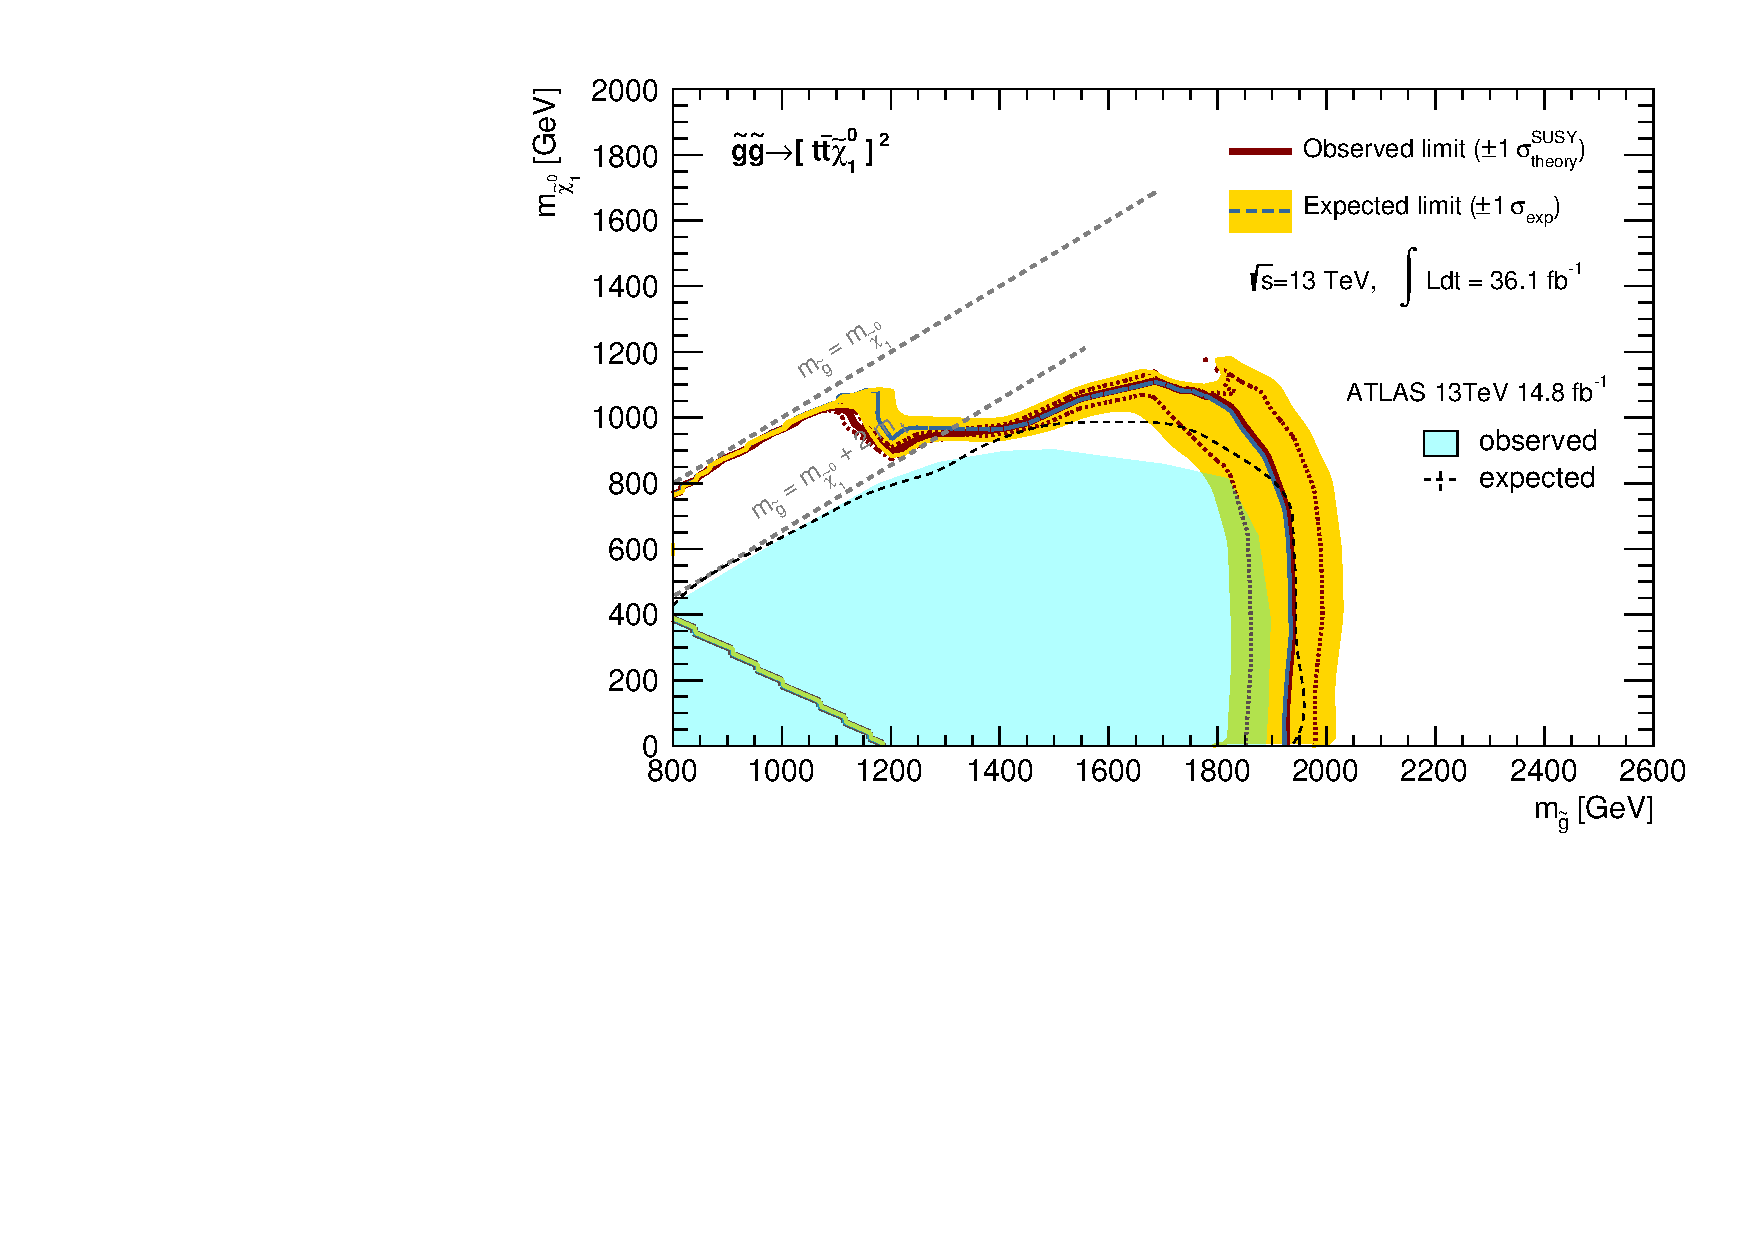
\includegraphics[width=140mm]{figures/Result/exclContour/atlascls_wband1_wfixSigXSecband1_showcms0_myAna_tag858_objRep_shapeSys_excl_GG_symTTN1_fixSigXSecNominal_x12_hypotest__1_harvest_list.pdf}
    \captionof{figure}{Exlusion limit for benchmark model \textbf{TTN1TTN1}.
      Observed limit is shown by the solid red line, while the expected limit are expressed by the dashed blue line with a yellow $1\sigma$ band. The past result provided by ATLAS (multi-$b$: \cite{strong3B_ICHEP2016_CONF}, same-sign leptons or three leptons: \cite{strongSS3L_ICHEP_CONF}) is overlayed (observed limit: magenta shade, expected limit: black dashed line), which is mostly given by the multi-$b$ analysis where the combination of 0-lepton and 1-lepton channel is performed. All limits correspond to 95$\%$ CL.
}
    \label{fig::Result::exclLimit::GG_ttn1}
  \end{center}
\end{figure}
%%%%%%%%%




\clearpage
%%%%%%%%%%%%
\paragraph{\underline{\textbf{Other benchmark models}}} \mbox{} \\ 
The exclusion limits for all the 45 models and grids are calculated similarly. 
Observed limits are compared in Figure \ref{fig::Result::combLimit::BV1}-\ref{fig::Result::combLimit::3B2}. 
BV/BT/3B benchmark models (defined respectively by Table \ref{tab::Introduction::modelsBV} - \ref{tab::Introduction::models3B}) are overlaid in the same plot respectively. 
Though the acceptance after the 1-lepton pre-selection are similar between them, the final sensitivity does vary depending on the branching into the 1-lepton final state which has a relatively wide variety. This ends up in $300\gev\sim400\gev$ of difference in gluino mass at the largest. On the other hand, this implies that the models with less sensitivity can be fully recovered by the combination with 0-lepton final state. Aside such several models with the small 1-lepton branches, the variation is typically $100\gev\sim200\gev$, which confirms the inclusiveness of the analysis.


%%%
%\clearpage
%-------------------------------
\begin{figure}[h]
  \centering
    \subfig{0.49}{figures/Result/combLimit/BV_x12_obs.pdf}{}
    \subfig{0.49}{figures/Result/combLimit/BV_varx_obs.pdf}{}
    \subfig{0.49}{figures/Result/combLimit/BV_dM20_obs.pdf}{}
    \subfig{0.49}{figures/Result/combLimit/BV_dM30_obs.pdf}{}
    \caption{
    Observed limit for BV benchmark moelds (defined in Table \ref{tab::Introduction::modelsBV}) presented in grid (a) $\xhalf$ (b) $\varx$ (c) $\DMtw$ (d) $\DMth$.
      \label{fig::Result::combLimit::BV1} }
\end{figure}
%-------------------------------


\clearpage
%-------------------------------
\begin{figure}[h]
  \centering
    \subfig{0.9}{figures/Result/combLimit/BT_x12_obs.pdf}{}
    \subfig{0.9}{figures/Result/combLimit/BT_varx_obs.pdf}{}
    \caption{
    Observed limit for BT benchmark models (defined in Table \ref{tab::Introduction::modelsBT}) presented in grid (a) $\xhalf$ (b) $\varx$.
      \label{fig::Result::combLimit::BT1} }
\end{figure}


\begin{figure}[h]
  \centering
    \subfig{0.9}{figures/Result/combLimit/BT_dM20_obs.pdf}{}
    \subfig{0.9}{figures/Result/combLimit/BT_dM30_obs.pdf}{}
    \caption{
    Observed limit for BT benchmark models (defined in Table \ref{tab::Introduction::modelsBT}) presented in grid (a) $\DMtw$ (b) $\DMth$.
      \label{fig::Result::combLimit::BT2} }
\end{figure}
%-------------------------------



\clearpage
%-------------------------------
\begin{figure}[h]
  \centering
    \subfig{0.9}{figures/Result/combLimit/3B_x12_obs.pdf}{}
    \subfig{0.9}{figures/Result/combLimit/3B_varx_obs.pdf}{}
    \caption{
    Observed limit for 3B benchmark models (defined in Table \ref{tab::Introduction::models3B}) presented in grid (a) $\xhalf$ (b) $\varx$.
      \label{fig::Result::combLimit::3B1} }
\end{figure}

\begin{figure}[h]
  \centering
    \subfig{0.9}{figures/Result/combLimit/3B_dM20_obs.pdf}{}
    \subfig{0.9}{figures/Result/combLimit/3B_dM30_obs.pdf}{}
    \caption{
    Observed limit for 3B benchmark models (defined in Table \ref{tab::Introduction::models3B}) presented in grid (a) $\DMtw$ (b) $\DMth$.
      \label{fig::Result::combLimit::3B2} }
\end{figure}
%-------------------------------




%%%%%%%%%%%%




\clearpage
\section{Obtained Cross-section Upper-limit}
$\mathrm{CL_s}$ value is calculated as the function of the signal strength $\mu (\in [0,5])$ in the hypothetical test. Therefore, the upper limit on $\mu$ can be determined as:
\begin{align}
\mu_{95\mathrm{CL}} := \mu(\mathrm{CL_s}=0.05).
\end{align}
This can be straightforwardly interpreted into the upper limit on the excluded cross-section ($\sigma_{95\mathrm{CL}}$), and it is a completely model-independent presentation of the result once the decay chain and the masses of gluino and EW-gauginos are specified.
Figure \ref{fig::Result::xsecUL::QQC1QQC1}-\ref{fig::Result::xsecUL::TTN1TTN1} present the results for the reference models \textbf{QQC1QQC1}, \textbf{QQC1BTC1} and \textbf{TTN1TTN1}. \\
%, and the full result are in the Appendix \ref{sec::Result::xsecUL::nonBenchMark}.

\clearpage
%% -- xsec UL ----------------------
\begin{figure}[h]
  \centering
%    \subfigure[]{\includegraphics[width=0.48\textwidth]{figures/Result/xsecUL/onestepCC_x12.pdf}}
%    \subfigure[]{\includegraphics[width=0.48\textwidth]{figures/Result/xsecUL/onestepCC_varx.pdf}}
    \subfigure[]{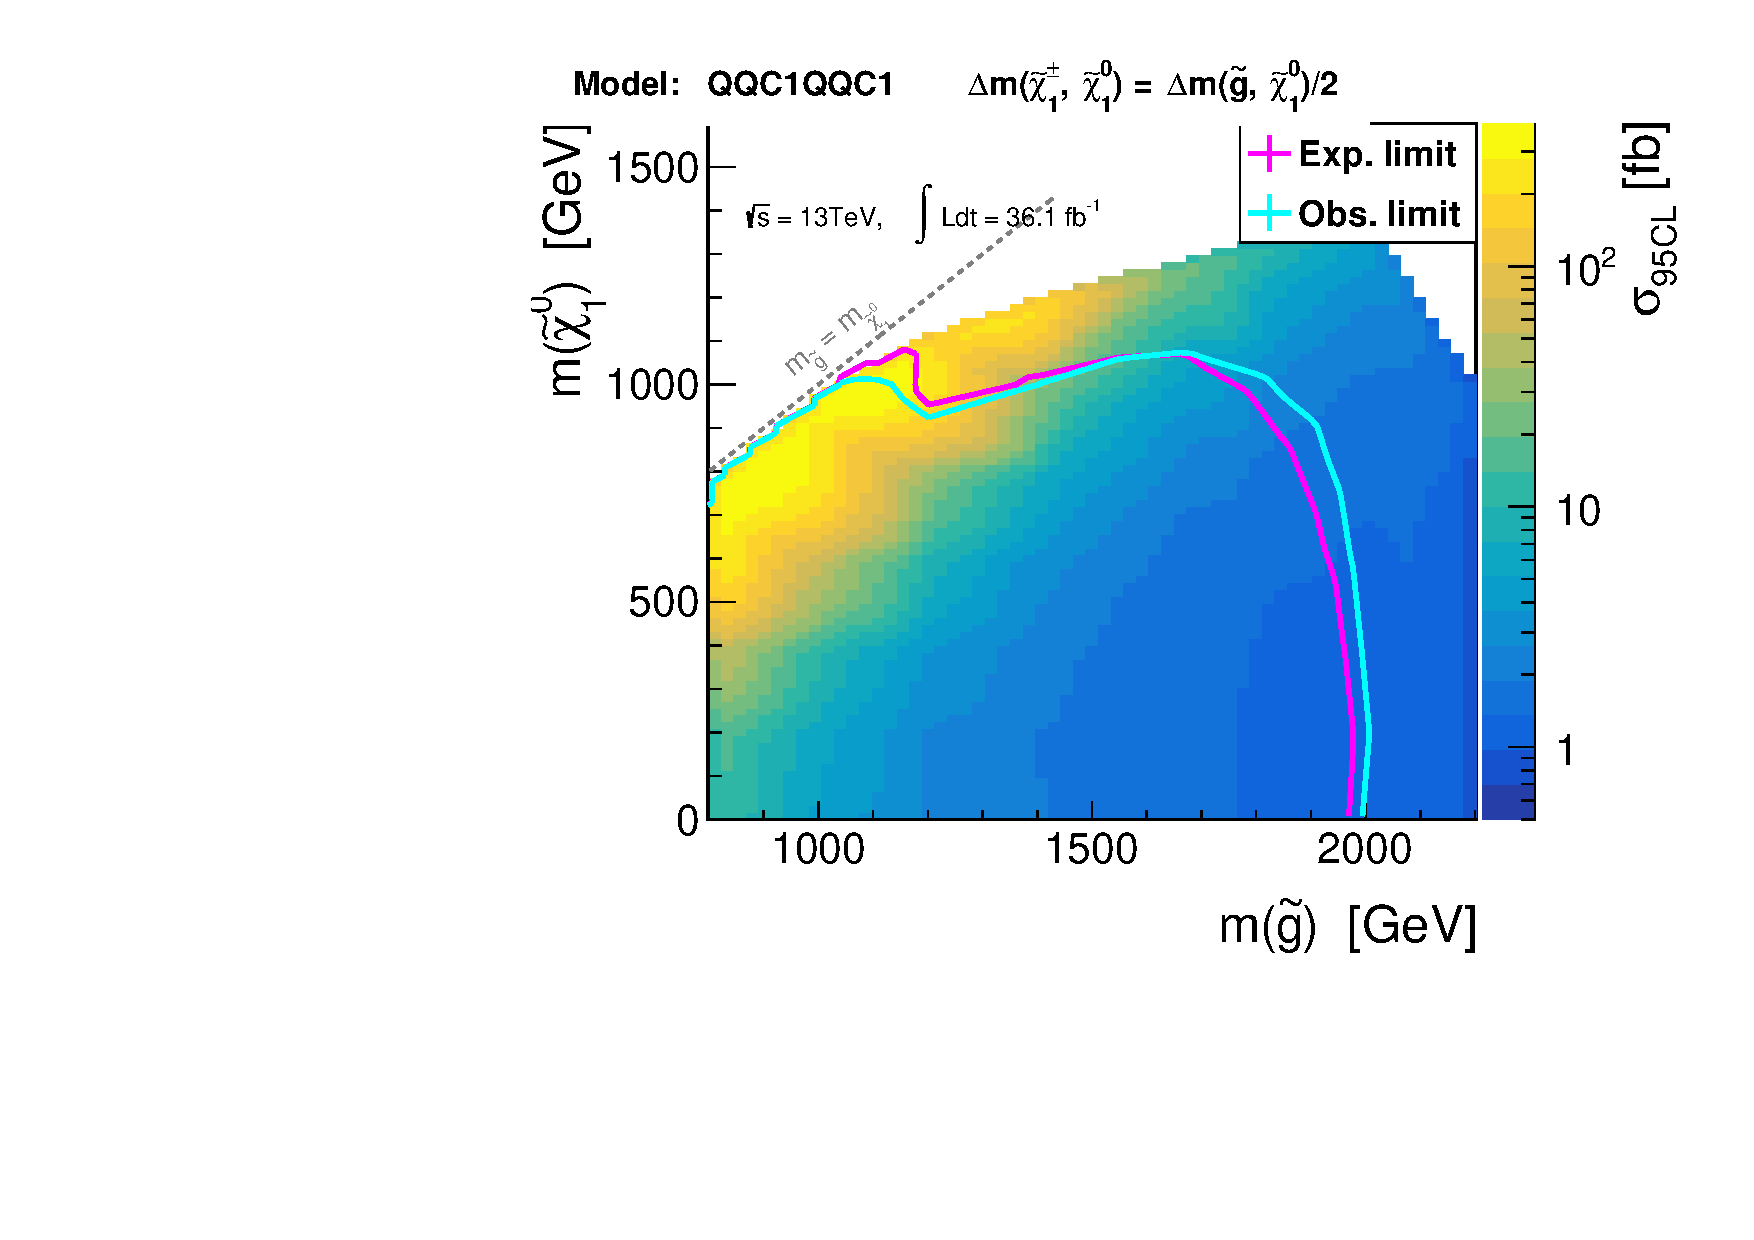
\includegraphics[width=0.48\textwidth]{figures/Result/xsecUL/symQQC1_x12.pdf}}
    \subfigure[]{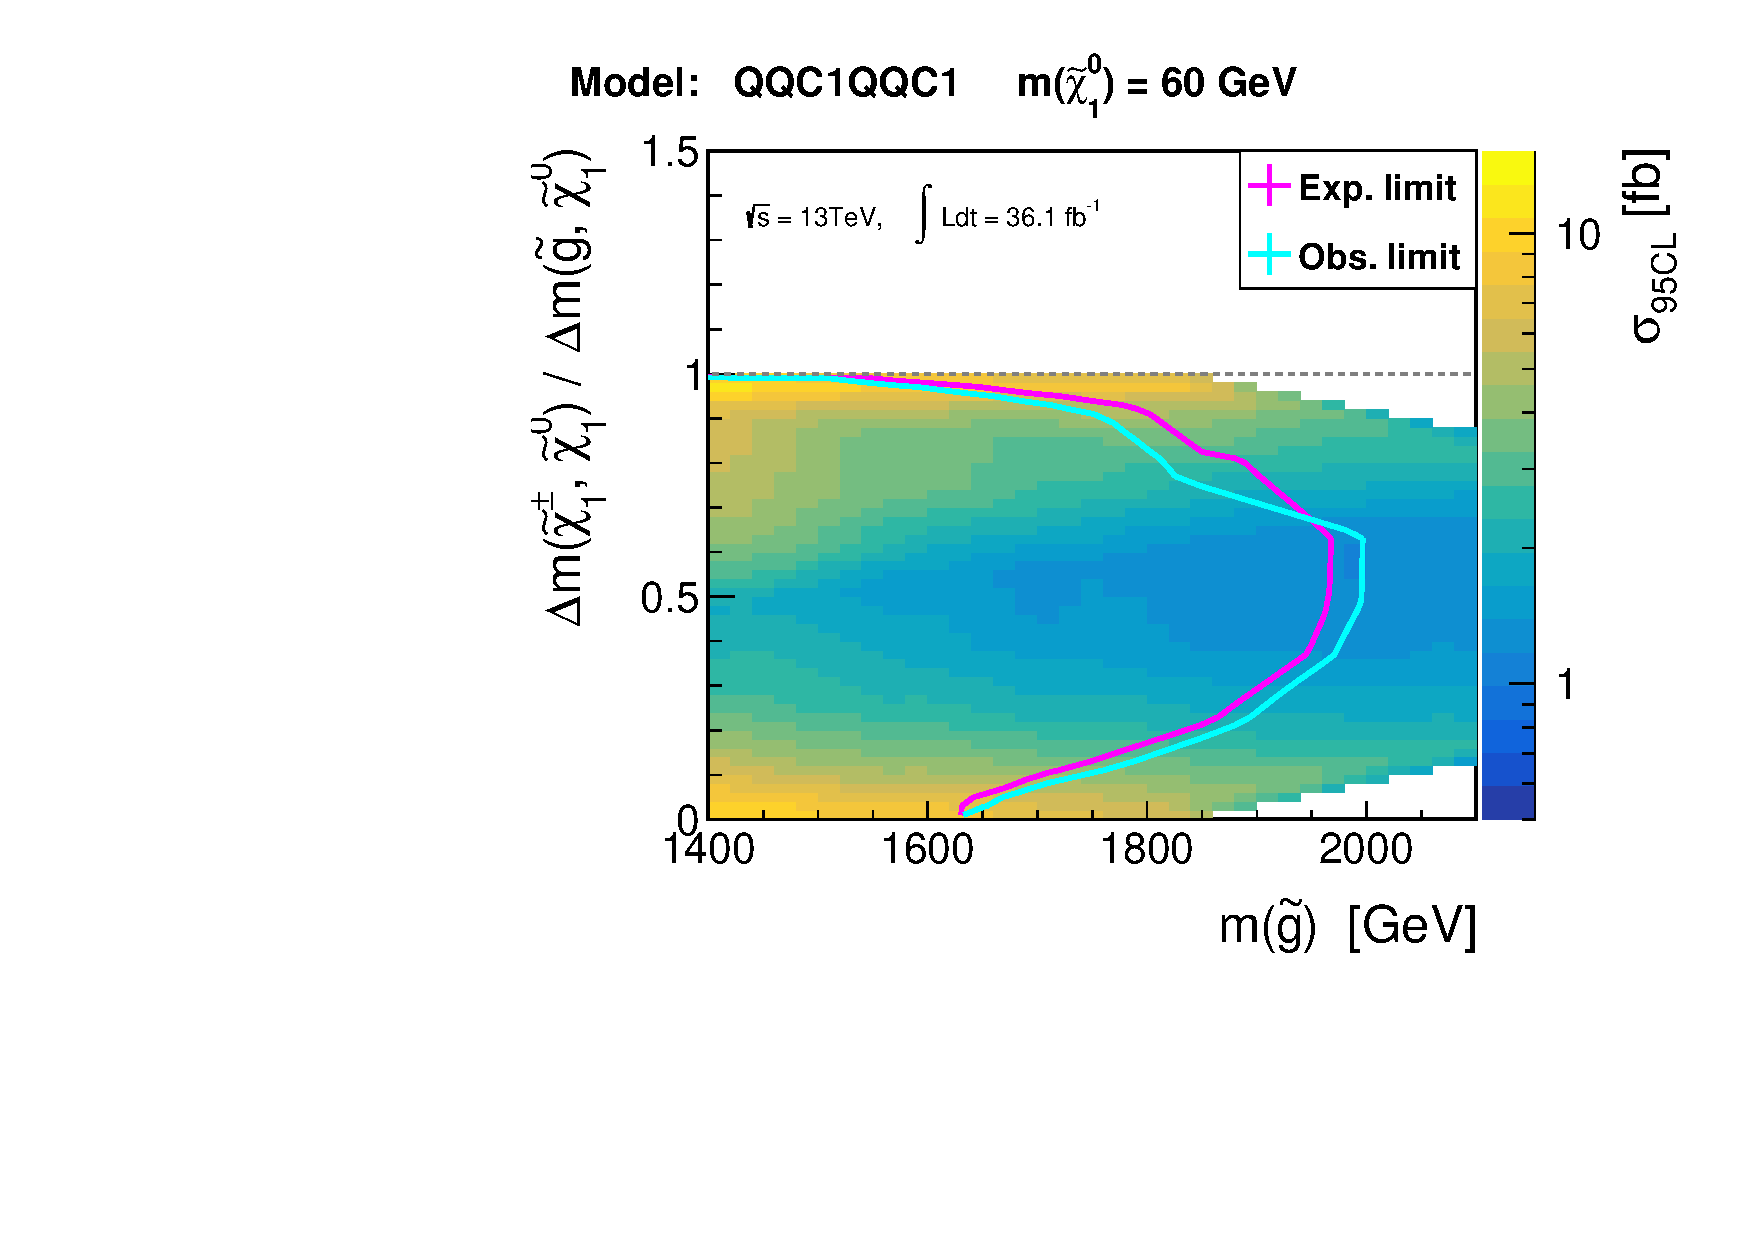
\includegraphics[width=0.48\textwidth]{figures/Result/xsecUL/symQQC1_varx.pdf}}
    \subfigure[]{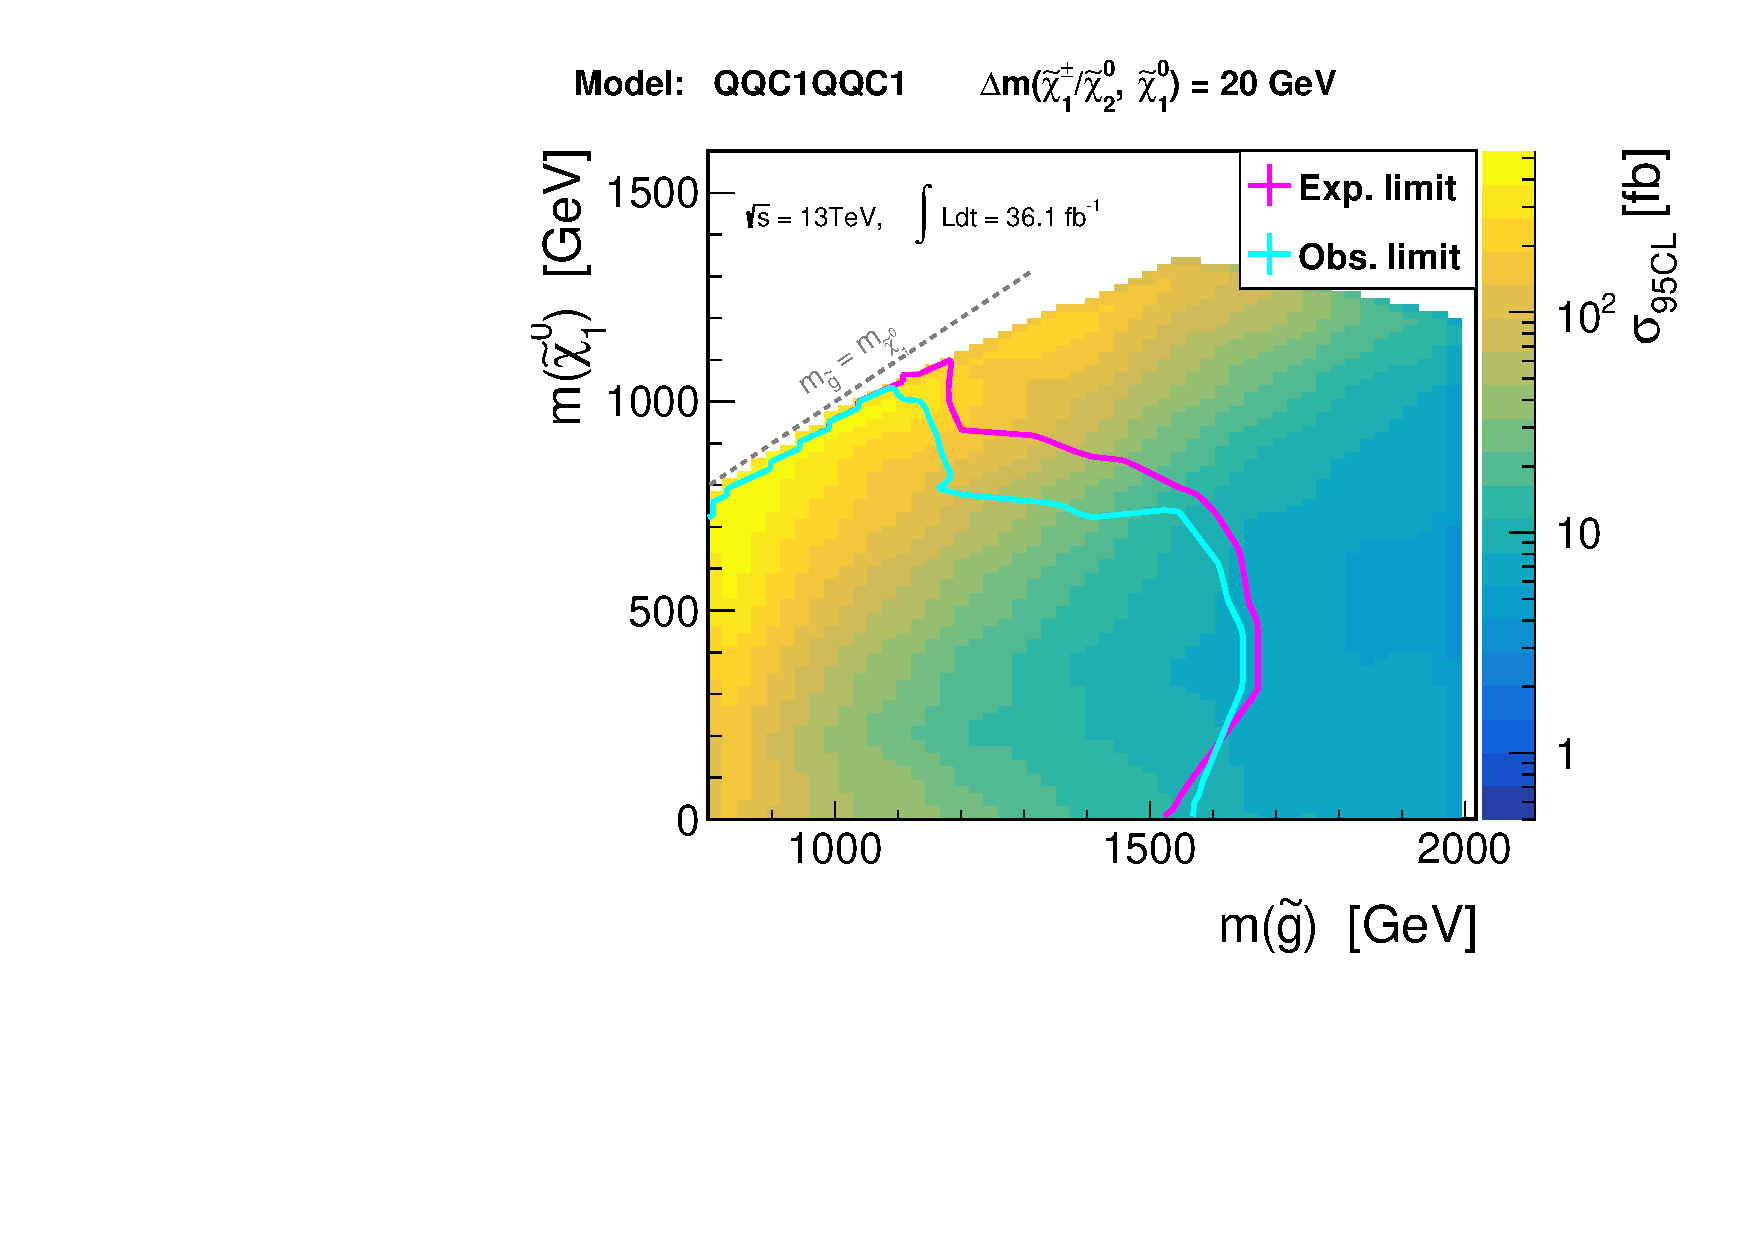
\includegraphics[width=0.48\textwidth]{figures/Result/xsecUL/symQQC1_dM20.pdf}}
    \subfigure[]{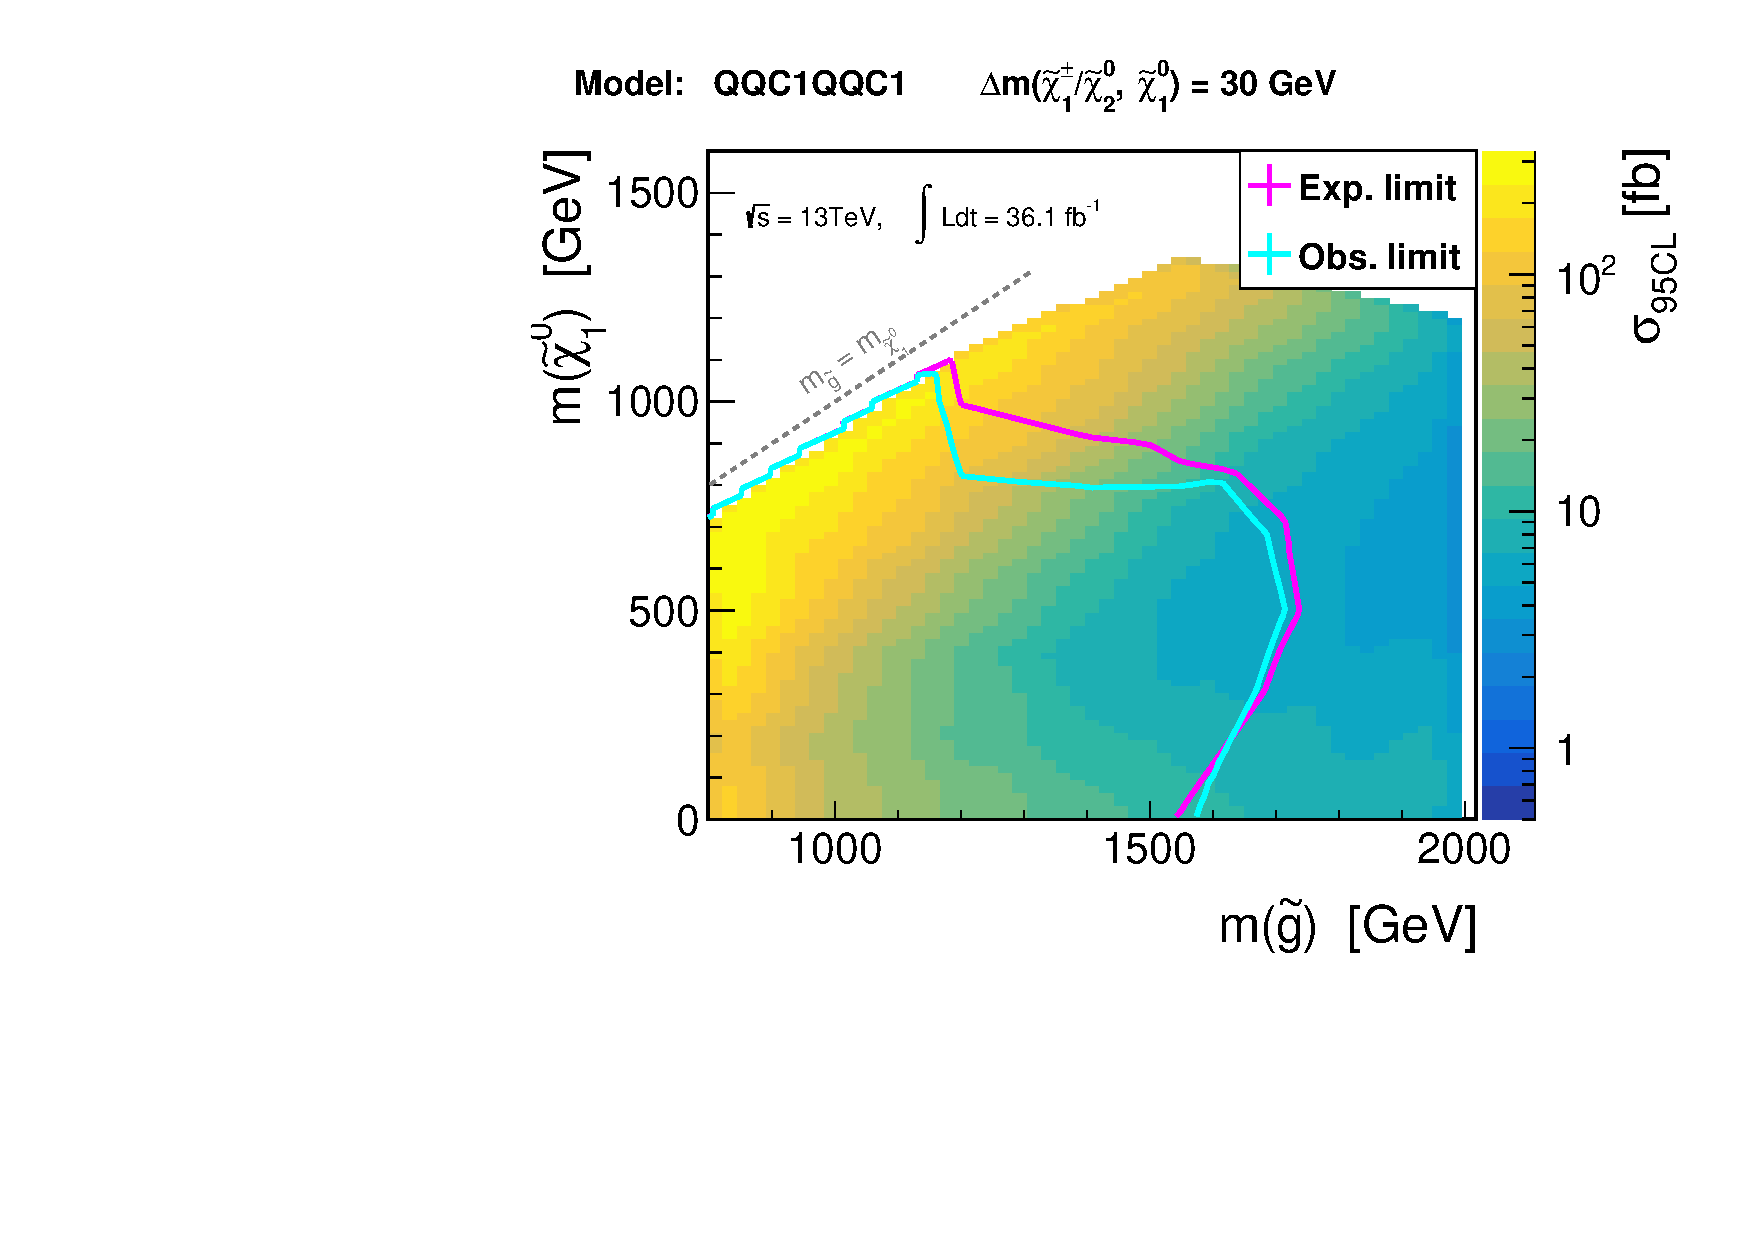
\includegraphics[width=0.48\textwidth]{figures/Result/xsecUL/symQQC1_dM30.pdf}}
    \caption{
    Upper limit of excluded cross-section (95$\%$CL) as the function of the SUSY masses, for benchmark model \textbf{QQC1QQC1}, presented in the grids (a) $x=1/2$ (b) $\mLSP=60\gev$ (c) $\dmc=20\gev$ (d) $\dmc=30\gev$.
    \label{fig::Result::xsecUL::QQC1QQC1} }
\end{figure}


%figures/Result/xsecUL/symQQC1_dM20.pdf

%% --
\begin{figure}[h]
  \centering
    \subfigure[]{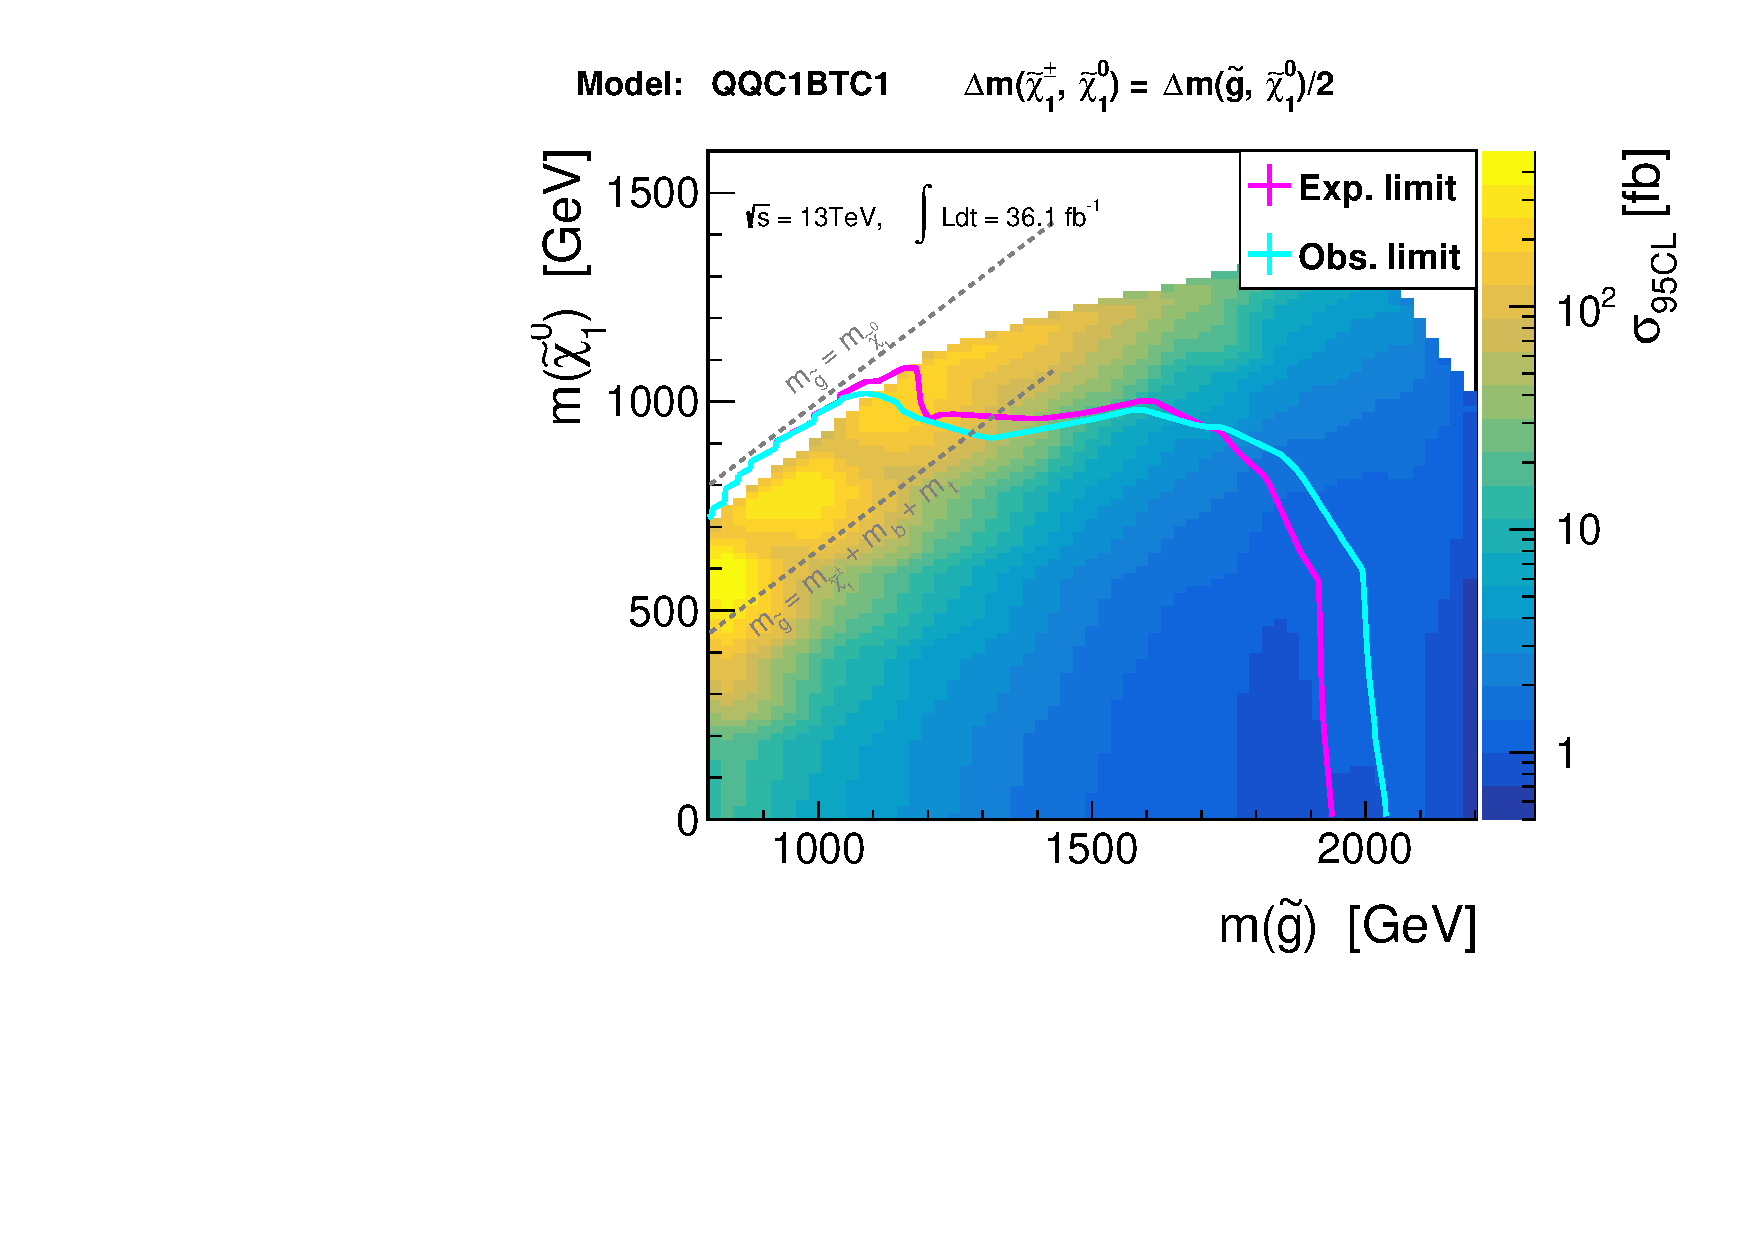
\includegraphics[width=0.48\textwidth]{figures/Result/xsecUL/QQC1BTC1_x12.pdf}}
    \subfigure[]{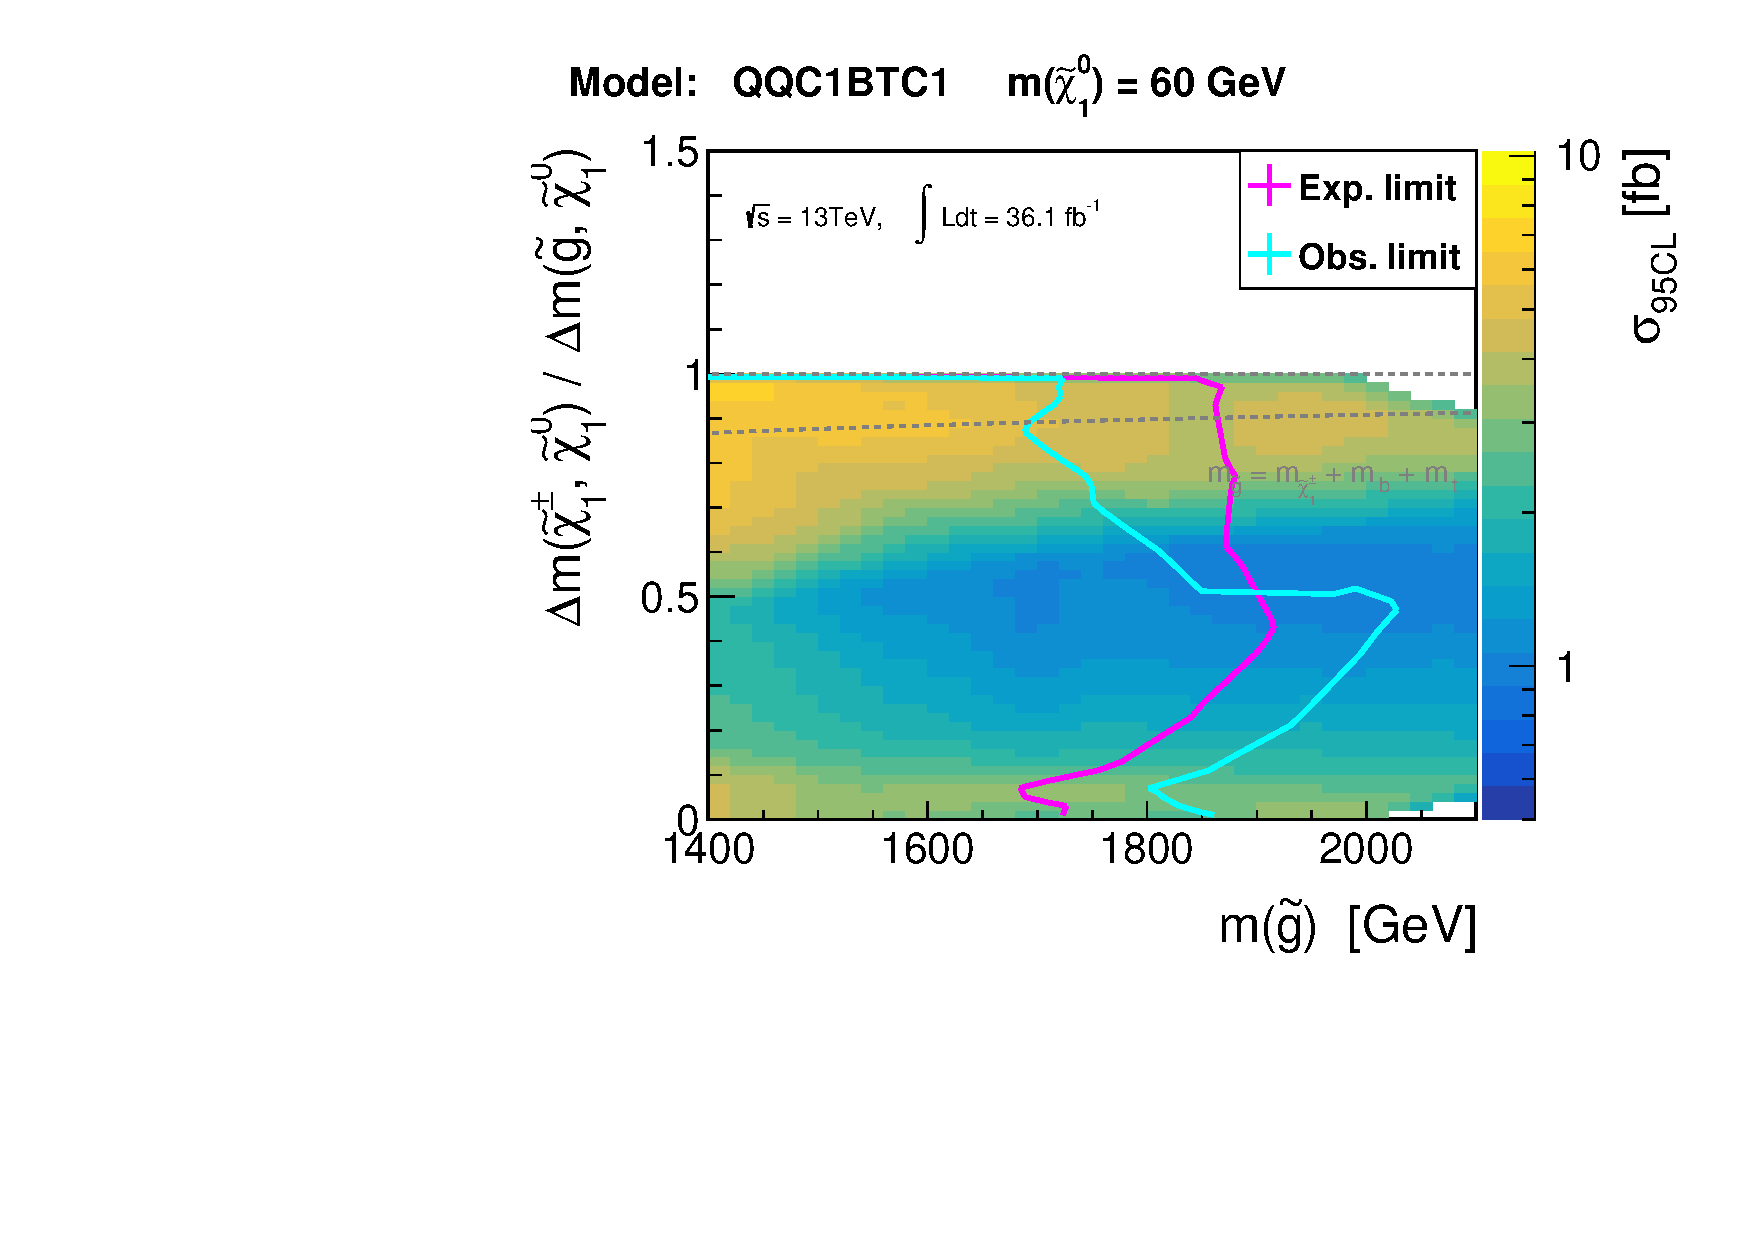
\includegraphics[width=0.48\textwidth]{figures/Result/xsecUL/QQC1BTC1_varx.pdf}}
    \subfigure[]{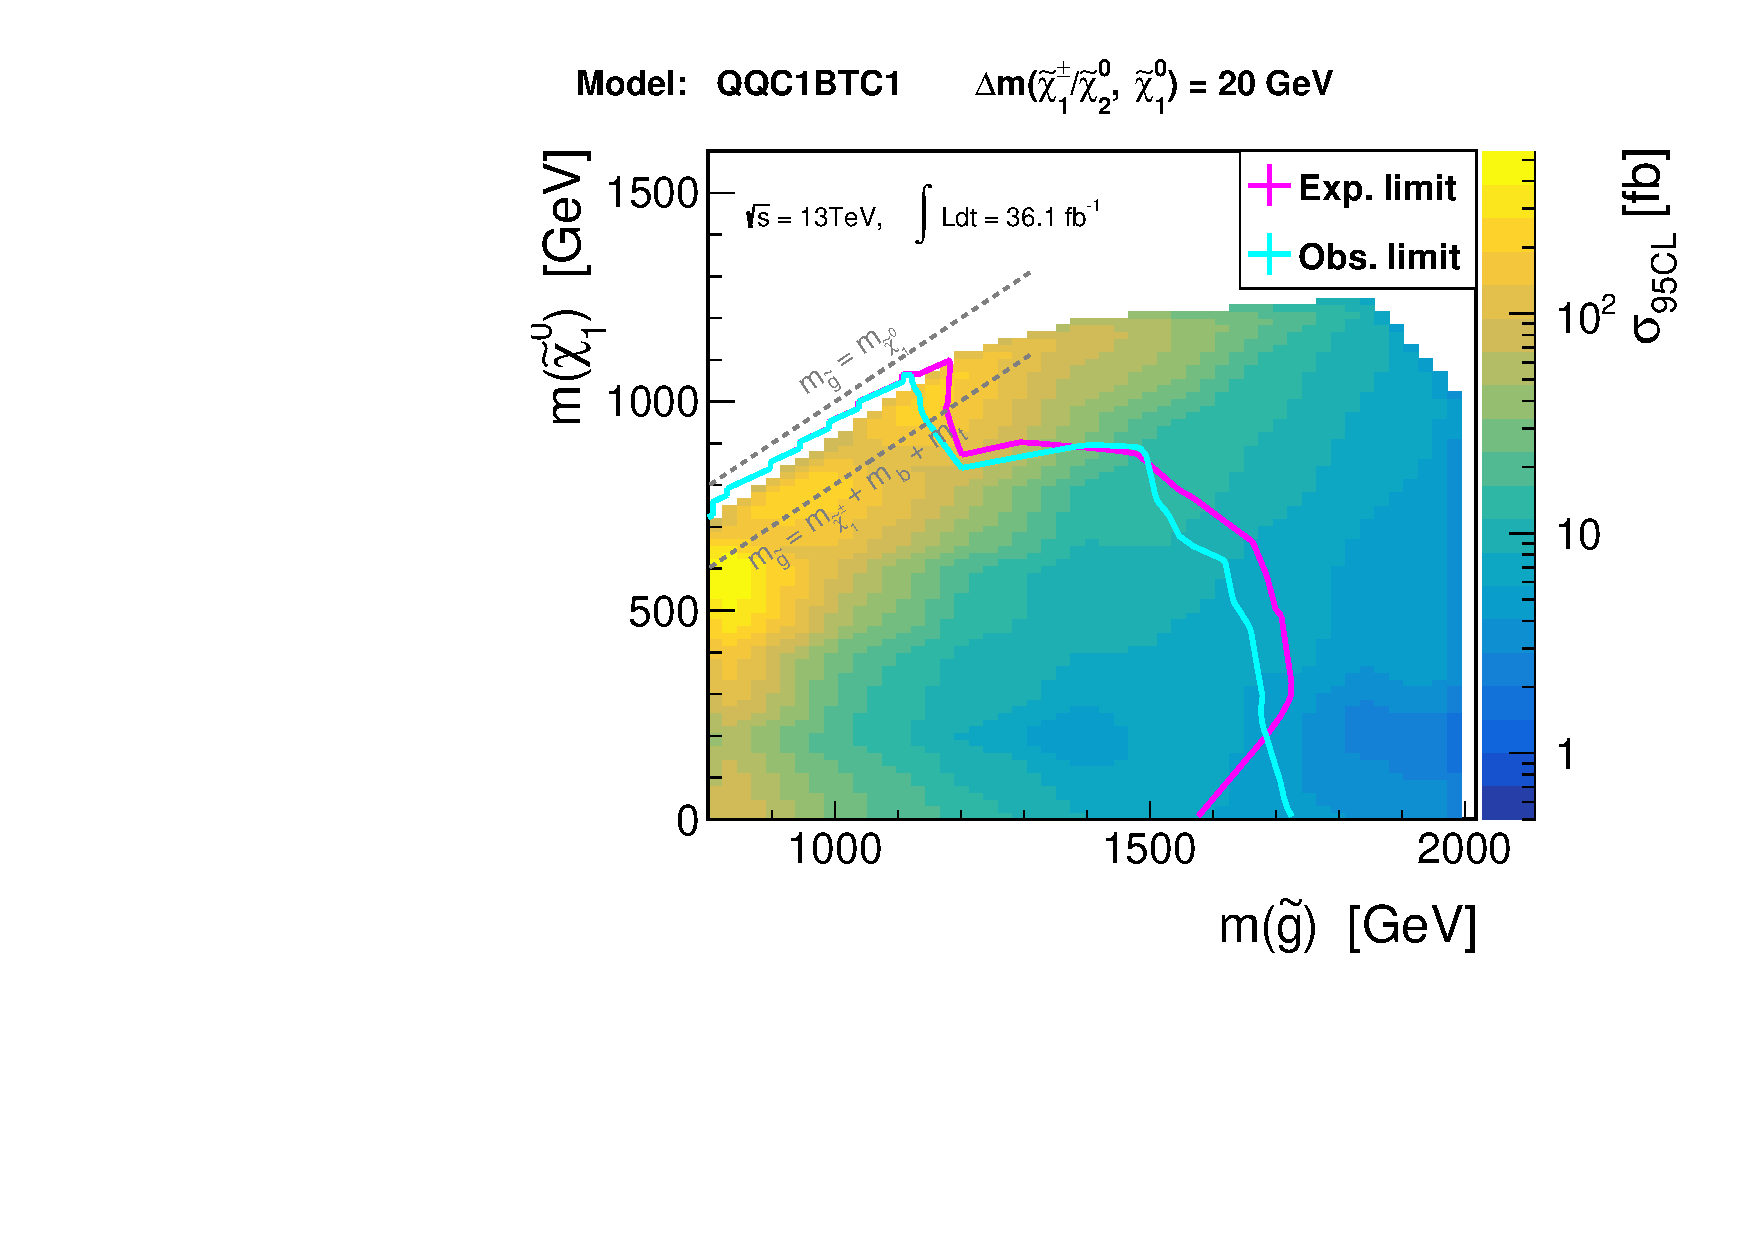
\includegraphics[width=0.48\textwidth]{figures/Result/xsecUL/QQC1BTC1_dM20.pdf}}
    \subfigure[]{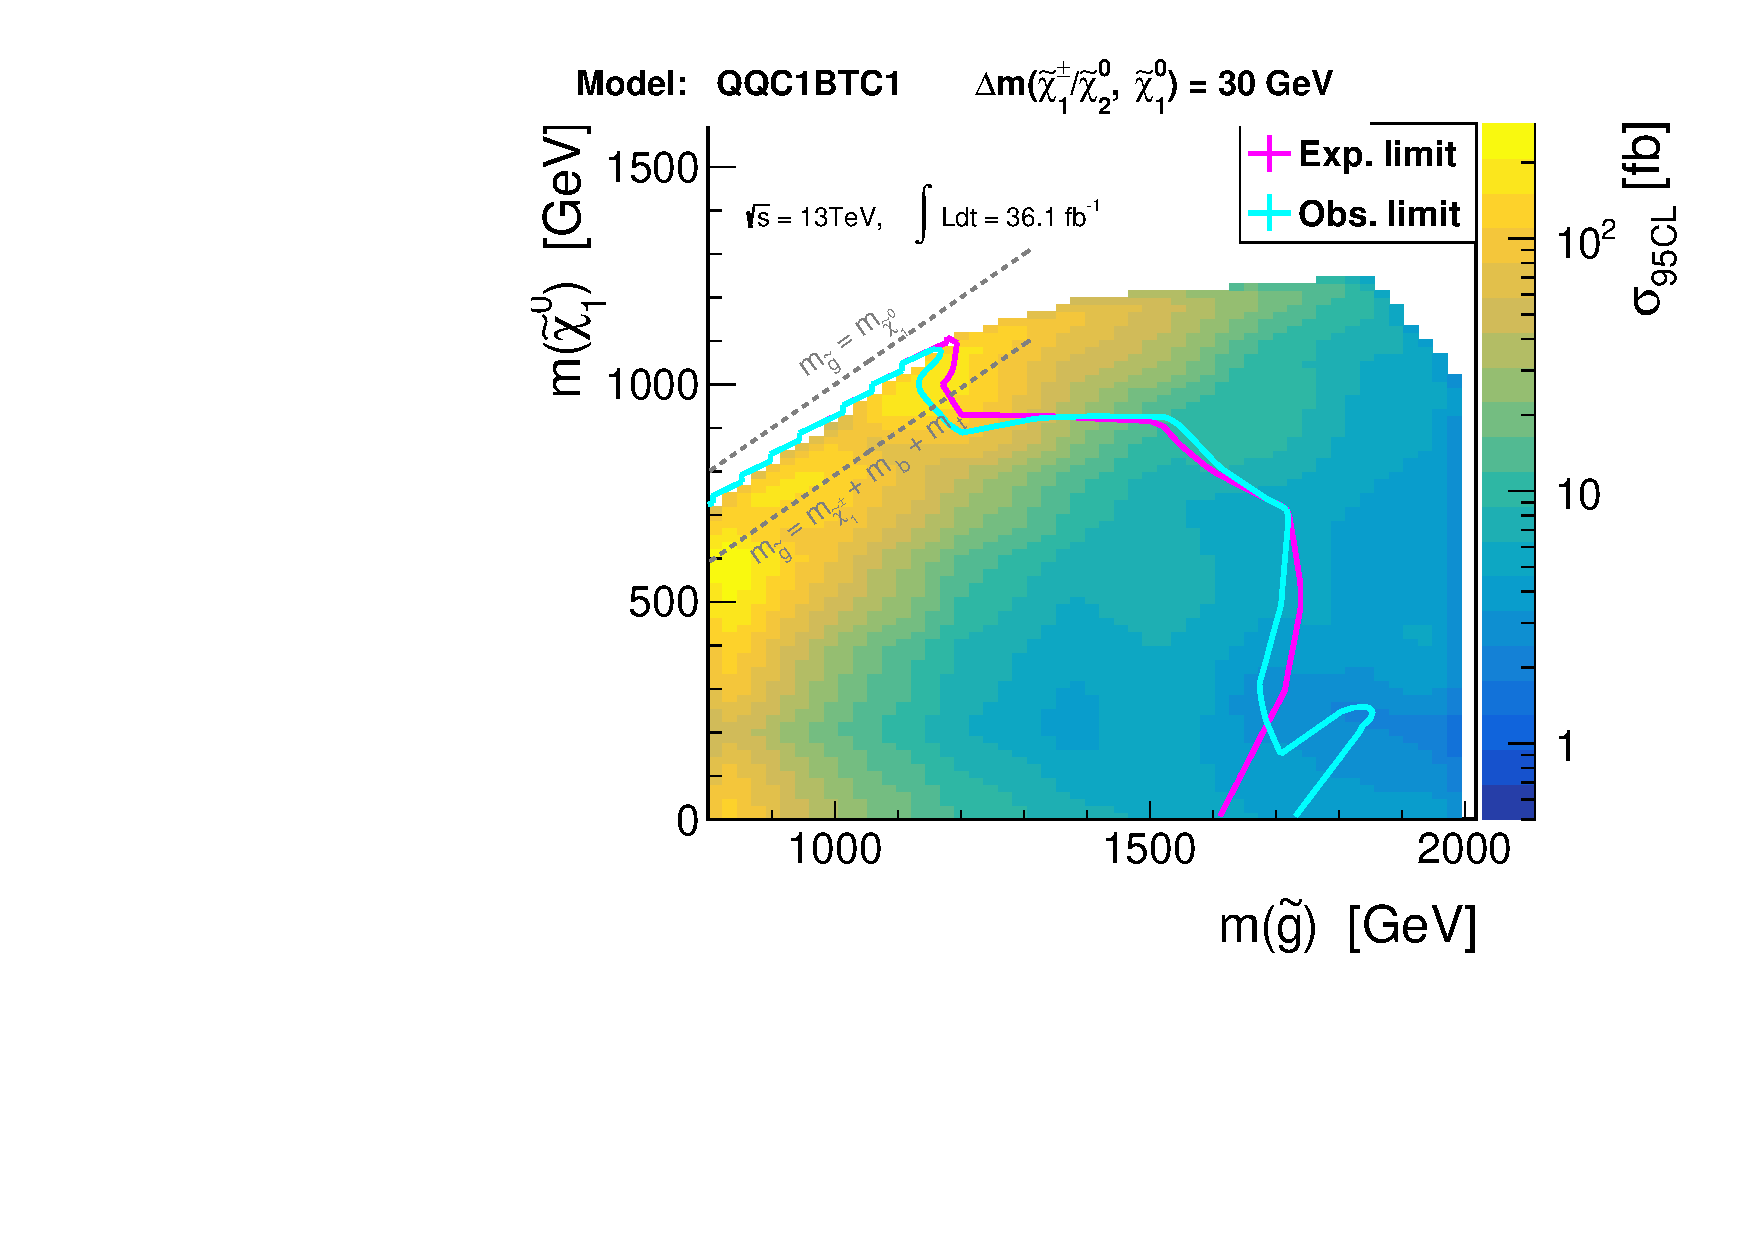
\includegraphics[width=0.48\textwidth]{figures/Result/xsecUL/QQC1BTC1_dM30.pdf}}
    \caption{
    Upper limit of excluded cross-section (95$\%$CL) as the function of the SUSY masses, for benchmark model \textbf{QQC1BTC1}, presented in the grids (a) $x=1/2$ (b) $\mLSP=60\gev$ (c) $\dmc=20\gev$ (d) $\dmc=30\gev$.
    \label{fig::Result::xsecUL::QQC1BTC1} }
\end{figure}

%% --
\begin{figure}
  \begin{center}
    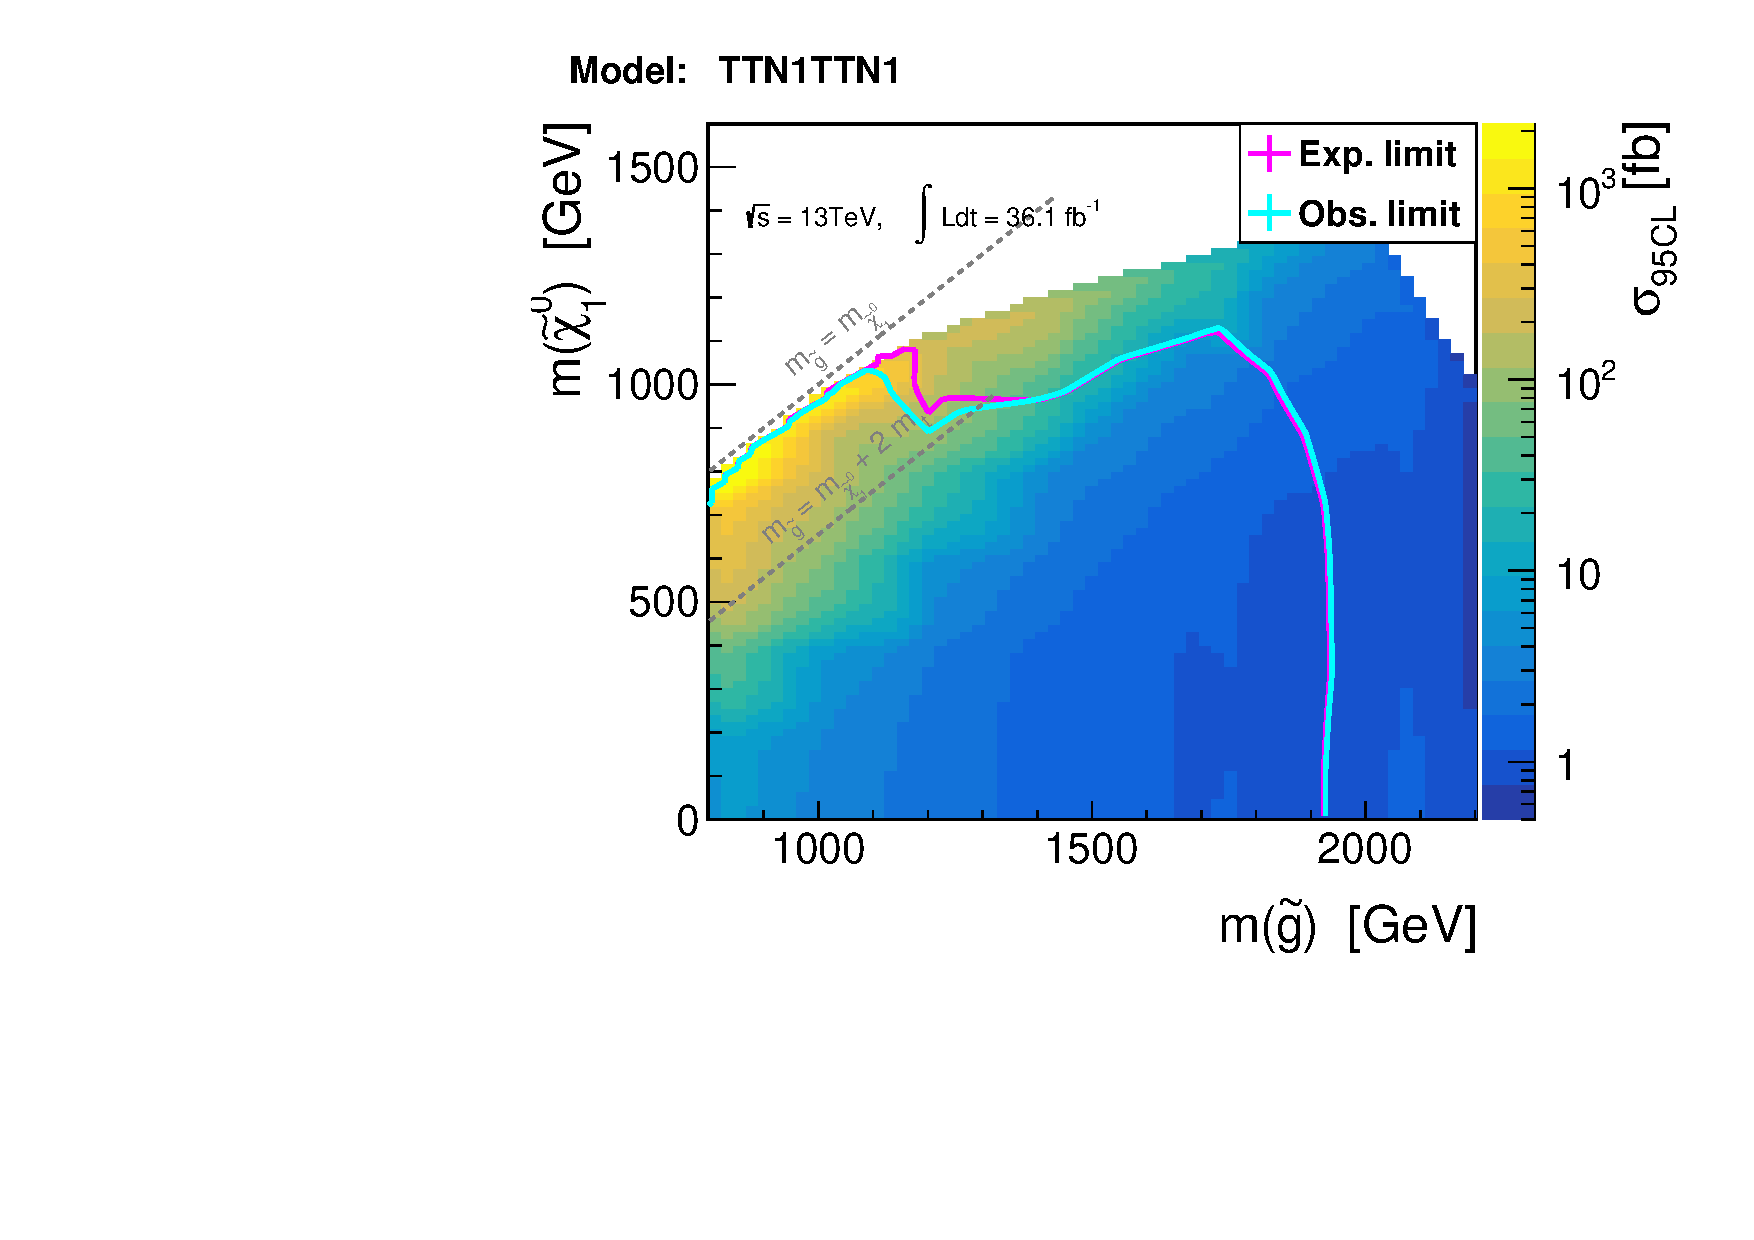
\includegraphics[width=160mm]{figures/Result/xsecUL/symTTN1_x12.pdf}
    \captionof{figure}{
    Upper limit of excluded cross-section (95$\%$CL) as the function of the SUSY masses, for benchmark model
 \textbf{TTN1TTN1}.
    \label{fig::Result::xsecUL::TTN1TTN1} }       
  \end{center}
\end{figure}
%-------------------------------                                                                                                   


